%%%%%%%%%%%%%%%%%%%%%%%% editor.tex %%%%%%%%%%%%%%%%%%%%%%%%%%%%%
%
% sample root file for the contributions of a "contributed volume"
%
% Use this file as a template for your own input.
%
%%%%%%%%%%%%%%%%%%%%%%%%%%%%% Springer %%%%%%%%%%%%%%%%%%%%%%%%%%


% RECOMMENDED %%%%%%%%%%%%%%%%%%%%%%%%%%%%%%%%%%%%%%%%%%%%%%%%%%%
\documentclass[graybox, envcountchap, twocolumn]{styles/svmult}

% general metadata:
\author{github.com/idf}
\title{Algorithm Quicksheet}
\subtitle{Classical equations, diagrams and tricks in algorithm}

% choose options for [] as required from the list
% in the Reference Guide

\usepackage{amssymb,amsmath,bm}
\DeclareMathAlphabet{\mathcal}{OMS}{cmsy}{m}{n}
\usepackage{textcomp}
\newcommand\abs[1]{\left\lvert#1\right\rvert}
\usepackage{longtable}
\usepackage{algorithm2e}
\usepackage{tocbibind}
\usepackage[toc]{multitoc}
\usepackage[utf8]{inputenc}

% Default fixed font does not support bold face
\DeclareFixedFont{\ttb}{T3}{txtt}{bx}{n}{8} % for bold
\DeclareFixedFont{\ttm}{T3}{txtt}{m}{n}{8}  % for normal

% Custom colors
\usepackage{color}
\definecolor{deepblue}{rgb}{0,0,0.5}
\definecolor{deepred}{rgb}{0.6,0,0}
\definecolor{deepgreen}{rgb}{0,0.5,0}

\usepackage{listings}

% Python style for highlighting
\newcommand\pythonstyle{
  \lstset{
    language=Python,
    basicstyle=\ttm,
    otherkeywords={assert, del},  % Add keywords here
    keywordstyle=\ttb\color{deepblue},
    columns=flexible,
    keepspaces=true,
    commentstyle=\ttm,
    emph={__init__},  % Custom highlighting
    emphstyle=\ttb\color{deepred},  % Custom highlighting style
    stringstyle=\color{deepgreen},
    % frame=tb,  % Any extra options here
    showstringspaces=false            
  }
}


% Python environment
\lstnewenvironment{python}[1][]{
  \pythonstyle
  \lstset{#1}
}{}

% Python for external files
\newcommand\pythonexternal[2][]{
  {
    \pythonstyle
    \lstinputlisting[#1]{#2}
  }
}

% Python for inline
\newcommand\pythoninline[1]{
  {
    \pythonstyle\lstinline!#1!
  }
}
\lstset{columns=fullflexible, commentstyle=\rm, basicstyle=\footnotesize} % remove columns=fullflexible for monospace

\renewcommand{\bibname}{References}
\usepackage{mathptmx}        % selects Times Roman as basic font
\usepackage{helvet}          % selects Helvetica as sans-serif font
\usepackage{courier}         % selects Courier as typewriter font
%\usepackage{type1cm}        % activate if the above 3 fonts are 
                             % not available on  your system

\usepackage{makeidx}         % allows index generation
\usepackage{graphicx}        % standard LaTeX graphics tool
                             % when including figure files
\usepackage[justification=centering]{caption}
\usepackage{subfig}
\usepackage{multicol}        % used for the two-column index
\usepackage{multirow}
\usepackage[bottom]{footmisc}% places footnotes at page bottom
\usepackage[bookmarksnumbered=true,
            bookmarksopen=true,
            colorlinks=true,
            linkcolor=blue,
            anchorcolor=blue,
            citecolor=blue
           ]{hyperref}

\graphicspath{{figures/}}

% see the list of further useful packages in the Reference Guide

\makeindex             % used for the subject index
                       % please use the style svind.ist with
                       % your makeindex program

%%%%%%%%%%%%%%%%%%%%%%%%%%%%%%%%%%%%%%%%%%%%%%%%%%%%%%%%%%%%%%%%%

\begin{document}

\frontmatter%%%%%%%%%%%%%%%%%%%%%%%%%%%%%%%%%%%%%%%%%%%%%%%%%%%%%%

\onecolumn
\begin{titlepage}

\begin{enumerate}
\item 
\begin{enumerate}
\item \begin{enumerate}
\item \begin{enumerate}
\item \begin{itemize}
\item text\end{itemize}\end{enumerate}\end{enumerate}\end{enumerate}
\end{enumerate}\url{https://github.com/algorhythms/Algo-Quicksheet}

\end{titlepage}

\newpage

\noindent \textcopyright  2015 github.com/idf \\
Except where otherwise noted, this document is licensed under a BSD 3.0
license (\url{http://opensource.org/licenses/BSD-3-Clause}).

%%%%%%%%%%%%%%%%%%%%%%% dedic.tex %%%%%%%%%%%%%%%%%%%%%%%%%%
%
% sample dedication
%
% Use this file as a template for your own input.
%
%%%%%%%%%%%%%%%%%%%%%%%% Springer %%%%%%%%%%%%%%%%%%%%%%%%%%

\begin{dedication}
This book is dedicated to all Software Engineers.
\end{dedication}




%\include{foreword}
%%%%%%%%%%%%%%%%%%%%%%preface.tex%%%%%%%%%%%%%%%%%%%%%%%%%%%%%%%%%%%%%%%%%
% sample preface
%
% Use this file as a template for your own input.
%
%%%%%%%%%%%%%%%%%%%%%%%% Springer %%%%%%%%%%%%%%%%%%%%%%%%%%

\preface

This quicksheet contains many classical equations and diagrams on algorithm, which will help you quickly recall knowledge and ideas in algorithm.\\

This quicksheet has three significant advantages:
\begin{enumerate}
\item Quick recall
\item Compact knowledge representation
\item Mathematical notations to increase information entropy per unit word. 
\end{enumerate}

\vspace{\baselineskip}
\begin{flushright}\noindent
At GitHub, June 2015\hfill {\it github.com/idf} \\
\end{flushright}



%\include{acknow}

\tableofcontents
%%%%%%%%%%%%%%%%%%%%clist.tex %%%%%%%%%%%%%%%%%%%%%%%%
%                                                    
% sample list of contributors and their addresses    
%                                                    
% Use this file as a template for your own input.    
%                                                    
%%%%%%%%%%%%%%%%%%%%%%%% Springer %%%%%%%%%%%%%%%%%%%%
\contributors

\begin{thecontriblist}
Daniel D. Zhang (\urld{github.com/idf})
\end{thecontriblist}

%%%%%%%%%%%%%%%%%%%%%%%acronym.tex%%%%%%%%%%%%%%%%%%%%%%%%%%%%%%%%%%%%%%%%%
% sample list of acronyms
%
% Use this file as a template for your own input.
%
%%%%%%%%%%%%%%%%%%%%%%%% Springer %%%%%%%%%%%%%%%%%%%%%%%%%%

\Extrachap{Acronym}

\runinhead{A} Array 
\runinhead{idx} Index
\runinhead{TLE} Time Limit Exceeded
\runinhead{MLE} Memory Limit Exceeded
\runinhead{dp} Dynamic programming 
\runinhead{def} Definition
\runinhead{ptr} Pointer 
\runinhead{$\pi$/pi} The parent of a child

\Extrachap{Notations}\label{sec:Notation}

\section*{General Math Notations}

\begin{longtable}{cl}
\hline\noalign{\smallskip}
\textbf{Symbol} & \textbf{Meaning} \\
\noalign{\smallskip}\hline\noalign{\smallskip}
$\lfloor x \rfloor$ & Floor of $x$, i.e. round down to nearest integer\\
$\lceil x \rceil$ & Ceiling of $x$, i.e. round up to nearest integer\\
floor(key) & the largest key $\leq$ the given key \\
ceil(key) & the smallest key $\geq$ the given key \\
$\log x$ & The base of logarithm is 2 unless otherwise stated\\
$a \wedge b$ & Logical AND\\
$a \vee b$ & Logical OR\\
$\neg a $ & Logical NOT\\
$a\AND b$ & Bit AND\\
$a \OR b$ & Bit OR\\
$a \XOR  a$ & Bit XOR\\
$\NOT a$ & Bit NOT\\
$\SHIFTL a$ & Bit shift left\\
$\SHIFTR a$ & Bit shift right\\
$\infty$ & Infinity\\
$\rightarrow$ & Tends towards, e.g., $n \rightarrow \infty$\\
$\propto$ &Proportional to; $y = ax$ can be written as $y \propto x$\\
$\abs{x}$ & Absolute value\\
$||\vec{a}||$ & $L_2$ distance (Euclidean distance) of a vector; norm-2 \\
$\abs{\mathcal{S}}$ & Size (cardinality) of a set\\
$n!$ & Factorial function\\
$\triangleq$ & Defined as\\
$O(\cdot)$ & Big-O: roughly means order of magnitude\\
$\mathbb{R}$ & The real numbers\\
$0:n$ & Range (Python convention): $0:n = {0, 1, 2,...,n-1}$\\
$\approx$ & Approximately equal to\\
$\sim$ & Tilde, the leading term of mathematical expressions \\
$\arg\max\limits_x f(x)$ & Argmax: the value $x$ that maximizes $f$\\
$\binom{n}{k}$ & $n$ choose $k$ , equal to $\frac{n!}{k!(n-k)!}$\\
$range(i,j)$ & range of number from i (inclusive) to j (exclusive) \\
$A[i:j]$ & subarray consist of $A_i, A_{i+1}, ..., A_{j-1}$.
\noalign{\smallskip}\hline\noalign{\smallskip}
\end{longtable}


\twocolumn



\mainmatter%%%%%%%%%%%%%%%%%%%%%%%%%%%%%%%%%%%%%%%%%%%%%%%%%%%%%%%
%\include{part}
% data structure 
\chapter{Basic Data  Structures}


\section{Introduction}
Abstract Data Types (ADT):
\begin{enumerate}
\item Queue
\item Stack
\item HashMap
\end{enumerate}
Implementation (for both queue and stack):
\begin{enumerate}
\item Linked List
\item Resizing Array:
\begin{enumerate}
\item Doubling: when full (100\%).
\item Halfing: when one-quarter full (25\%). 
\end{enumerate}}
\end{enumerate}}
Python Library:
\begin{enumerate}
\item \pythoninline{collections.deque} \footnote{The naming in Python collections is awkward: \href{http://stackoverflow.com/questions/18953681/naming-convention-in-collections-why-are-some-lowercase-and-others-capwords}{discussion}.}
\item \pythoninline{list}
\item \pythoninline{dict, OrderedDict, defaultdict}
\end{enumerate}} 
Java Library:
\begin{enumerate}
\item \javainline{java.util.Stack<E>}
\item \javainline{java.util.LinkedList<E>}
\item \javainline{java.util.HashMap<K, V>; java.util.TreeMap<K, V>}
\end{enumerate}}

\section{Stack}
\subsection{Stack and Recursion}
How a compiler implements a function:
\begin{enumerate}
\item Function call: push local environment and return address
\item Return: pop return address and local environment. 
\end{enumerate}

Recursive function: function calls itself. It can always be implemented by using an explicit stack to remove recursion. 

Stack can convert recursive \textbf{dfs} to iterative. 

\subsection{Usage}
The core philosophy of using stack is to maintain a relationship invariant among stack element. 

The \textbf{relationship invariants} can be:
\begin{enumerate}
\item strictly asc/ strictly desc
\item non-desc/ non-asc
\end{enumerate}

\subsection{Applications}
\runinhead{Largest Rectangle.} Find the largest rectangle in the matrix (histogram). Given $n$ non-negative integers representing the histogram's bar height where the width of each bar is 1, find the area of largest rectangle in the histogram. 

\begin{figure}[hbtp]
\centering
\subfloat{\includegraphics[scale=2.00]{histogram_area}}
\caption{Largest rectangle in histogram}
\label{fig:histogram_area}
\end{figure}

Keep a stack storing the bars in non-decreasing, then calculate the area by popping out the stack to get the currently lowest bar which determines the height of the rectangle.
\\
Core clues:
\begin{enumerate}
\item \textbf{Invariant}: Maintain the non-decreasing stack, using INDEX.
\item Popping triggers the calculation of area
\item Calculate the rectangle width by index diff
\item Post-processing in the end
\end{enumerate}
\newpage
Code:
\begin{python}
def largestRectangleArea(self, height):
    n = len(height)
    gmax = -sys.maxint-1
    stk = []  # store the idx, non-decreasing stack

    for i in xrange(n):
        while stk and height[stk[-1]] > height[i]:
            last = stk.pop()
            if stk:  # calculate area when popping
                area = height[last]*(i-(stk[-1]+1))
            else:
                area = height[last]*i
            gmax = max(gmax, area)

        stk.append(i)

    # after array scan, process the dangling stack
    i = n
    ...

    return gmax
\end{python}

\runinhead{Longest Valid Parentheses.} 
Given a string containing just the characters `(' and `)', find the length of the longest valid (well-formed) parentheses substring. Core clues:
\begin{enumerate}
\item \textbf{Invariant}: Stack holds the INDEX of UNPAIRED brackets, either ( or ).
\item Thus, \pyinline{stk[-1]} stores the last unpaired bracket. 
\item The length of the well-formed parentheses is: if currently \textbf{valid}, current scanning index \pyinline{idx} minus the last \textbf{invalid} index of bracket \pyinline{stk[-1]}
\end{enumerate}
\begin{python}
def longestValidParentheses(self, s):
  stk = []
  maxa = 0
  for idx, val in enumerate(s):
    if val == ")" and stk and s[stk[-1]] == "(":
      stk.pop()
      if not stk:
        maxa = max(maxa, idx+1)
      else:
        maxa = max(maxa, idx-stk[-1])
    else:
      stk.append(idx)

  return maxa

\end{python}
\subsection{All nearest smaller values}\label{allNearestSmaller}
\textbf{Nearest smaller}. Left neighbor of a value $v$ to be the value that occurs prior to $v$, is smaller than $v$, and is closer in position to $v$ than any other smaller value.

For each position in a sequence of numbers, search among the \textit{previous} positions for the last position that contains a smaller value. 

Core clues:
\begin{enumerate}
\item Nearest $\equiv$ spactial locality.
\item \textbf{Invariant}: Maintain a \textit{strictly increasing} stack.  
\item If all nearest \textit{larger} values, maintain a \textit{strictly decreasing} stack.  
\end{enumerate}

\begin{python}
def allNearestSmaller(self, A):
    P = [-1 for _ in A]
    stk = []
    for i, v in enumerate(A):
        while stk and A[stk[-1]] >= v: stk.pop()

        if stk:
            P[i] = stk[-1]
        else:
            P[i] = -1  # no preceding smaller value
            
        stk.append(i)  # store the idx or val

    return P
\end{python}

\section{Map}
\subsection{Math relations}
\textbf{1-1 Map}. Mathematically, full projection. One map, dual entries.
\begin{python}
class OneToOneMap(object):
    def __init__(self):
        self.m = {}  # keep a single map

    def set(self, a, b):
        self.m[a] = b
        self.m[b] = a

    def get(self, a):
        return self.m.get(a)
\end{python}
\subsection{Operations}
\runinhead{Sorting by value.} Sort the map entries by values \pyinline{itemgetter}.
\begin{python}
from operators import itemgetter 
sorted(hm.items(), key=itemgetter(1), reverse=True)
sorted(hm.items(), key=lambda x: x[1], reverse=True)
\end{python}

\chapter{Linked List}


\section{Operations}
\subsection{Fundamentals}
Get the $pre$ reference:
\begin{python}
dummy = Node(0)
dummy.next = head
pre = dummy
cur = pre.next
\end{python}

\subsection{Basic Operations}
\begin{enumerate}
\item Get the length
\item Get the $i$-th object
\item Delete a node 
\item Reverse
\begin{figure}[]
\centering
\subfloat{\includegraphics[scale=1.0]{ll_reverse}}
\caption{Reverse the linked list}
\label{fig:LABEL}
\end{figure}
\begin{python}
def reverseList(self, head):
    dummy = ListNode(0)
    dummy.next = head

    pre = dummy
    cur = pre.next
    while pre and cur:
        pre, cur.next, cur = cur, pre, cur.next
        # incorrect evaluation order:
        # pre, cur, cur.next = cur, cur.next, pre 

    dummy.next.next = None  # original head
    return pre  # new head
\end{python}
Notice: the evaluation order for the swapping the nodes and links. 
\end{enumerate}

\subsection{Combined Operations}
In $O(n)$ without extra space:
\begin{enumerate}
\item Determine whether two lists intersects
\item Determine whether the list is palindrome 
\item Determine whether the list is acyclic
\end{enumerate}

\section{Combinations}
\subsection{LRU}
Core clues:
\begin{enumerate}
\item Ensure $O(1)$ find $O(1)$ deletion. 
\item Doubly linked list + map.
\item Keep both \pyinline{head} and \pyinline{tail} pointer.
\item Operations on doubly linked list are case by case.  
\end{enumerate}
\begin{python}
class Node(object):
    def __init__(self, key, val):
        self.key = key
        self.val = val
        self.pre, self.next = None, None


class LRUCache(object):
    def __init__(self, capacity):
        self.cap = capacity
        self.map = {}  # key to node
        self.head = None
        self.tail = None

    def get(self, key):
        if key in self.map:
            cur = self.map[key]
            self._elevate(cur)
            return cur.val

        return -1

    def set(self, key, value):
        if key in self.map:
            cur = self.map[key]
            cur.val = value
            self._elevate(cur)
        else:
            cur = Node(key, value)
            self.map[key] = cur
            self._appendleft(cur)

            if len(self.map) > self.cap:
                last = self._pop()
                del self.map[last.key]

    # doubly linked-list operations only
    def _appendleft(self, cur):
        """Normal or initially empty"""
        if not self.head and not self.tail:
            self.head = cur
            self.tail = cur
            return

        head = self.head
        cur.next, cur.pre, head.pre = head, None, cur
        self.head = cur

    def _pop(self):
        """Normal or resulting empty"""
        last = self.tail
        if self.head == self.tail:
            self.head, self.tail = None, None
            return last

        pre = last.pre
        pre.next = None
        self.tail = pre
        return last

    def _elevate(self, cur):
        """Head, Tail, Middle"""
        pre, nxt = cur.pre, cur.next
        if not pre:
            return
        elif not nxt:
            assert self.tail == cur
            self._pop()
        else:
            pre.next, nxt.pre = nxt, pre

        self._appendleft(cur)
\end{python}

\chapter{Heap}


\section{Introduction}
Queue, Stack

\section{Python}
Python only has built in min-heap. To use max-heap, you can: 
\begin{enumerate}
\item Revert the number: 1 becomes -1.
\item Wrap the data into another class and override \_\_cmp\_\_ or \_\_lt\_\_
\end{enumerate}

The following code presents the wrapping method:
\begin{lstlisting}[language=python]
class Value(object):
    def __init__(self, val):
        self.val = val
        self.deleted = False  # lazy delete 

    def __cmp__(self, other):
        # Reverse order by height to get max-heap
        assert isinstance(other, Value)
        return other.val - self.val
\end{lstlisting}

Normally the deletion by value in Python is $O(n)$, to achieve $O(\lg n)$ we can use lazy deletion. Before take the top of the heap, we do the following:
\begin{lstlisting}[language=python]
while heap and heap[0].deleted:
    heapq.heappop(heap)
\end{lstlisting}
\subsection{Summarizing properties}



\chapter{Tree}

\section{Binary Tree}
\subsection{Introductions}
\runinhead{Get parent ref.} To get a parent reference (implicitly), \textit{return the Node} of the current recursion function to its parent to maintain the path. Sample code:
\begin{java}
Node deleteMin(Node x) {
    if (x.left == null) return x.right;
    x.left = deleteMin(x.left);
    // x.count = 1+size(x.left)+size(x.right);
    return x;
}
\end{java}
\runinhead{Construct path from root to target.} To search a node in binary tree (not necessarily BST), use dfs:
\begin{python}
def dfs(self, root, t, path, found):
    # post-call check
    if not root: return        
    if found[0]: return 

    path.append(root)
    if root == t:
        found[0] = True

    self.dfs(root.left, t, path, found)
    self.dfs(root.right, t, path, found)
    if not found[0]:
        path.pop()  # 1 pop() corresponds to 1 append()
\end{python}
The `found` is a wrapper for boolean to keep it referenced by all calling stack. 

\runinhead{Lowest common ancestor.} In BST, the searching is straightforward. In normal binary tree, construct the path from root to $node_1$ and $node_2$ respectively, and \textbf{diff} the two paths.

\runinhead{Find all paths.} Find all paths from root to leafs. For every currently visiting node, add itself to path; search left, search right and pop itself. Record current result when reaching the leaf.
\begin{python}
def dfs_path(self, cur, path, ret):
    if not cur: return

    path.append(cur)
    if not cur.left and not cur.right:
        ret.append("->".join(map(lambda x: str(x.val), path)))

    self.dfs_path(cur.left, path, ret)
    self.dfs_path(cur.right, path, ret)
    path.pop()
\end{python}
\subsection{Morris Traversal} 
Traversal with O(1) space. \footnote{\href{http://www.cnblogs.com/AnnieKim/archive/2013/06/15/MorrisTraversal.html}{ref}}

Time complexity $O(3n).$ - find \pyinline{pre} twice, \pyinline{cur} traverse once. \begin{figure}[hbtp]
\centering
\subfloat{\includegraphics[height=0.9in]{morris_time}}
\caption{Morris traversal time complexity}
\label{fig:morrisTime}
\end{figure}

\subsubsection{Inoder}
Assign the current node's in-order predecessor's right child to itself (threading). Two ptr \pyinline{cur}, \pyinline{pre}. 

Process:
\begin{enumerate}
\item If no left, \textit{consume} \pyinline{cur}, go right 
\item If left, find in-order predecessor \pyinline{pre}
\begin{enumerate}
\item If no thread (i.e. no \pyinline{pre} right child), assign it to \pyinline{cur}; go left
\item If thread, \textit{consume} \pyinline{cur}, go right. ($\equiv$ no left). 
\end{enumerate}
\end{enumerate}

\begin{figure}[hbtp]
\centering
\subfloat{\includegraphics[height=1.6in]{morris_inorder}}
\caption{Morris inorder traversal}
\label{fig:morrisInorder}
\end{figure}
\newpage
Code:
\begin{python}
def morris_inorder(self, root):
    cur = root
    while cur:
        if not cur.left:
            self.consume(cur)
            cur = cur.right
        else:
            pre = cur.left
            while pre.right and pre.right != cur:
                pre = pre.right

            if not pre.right:
                pre.right = cur
                cur = cur.left
            else:
                pre.right = None
                self.consume(cur)
                cur = cur.right
\end{python}
\subsubsection{Preoder}
Similar to inorder. 

Process:
\begin{enumerate}
\item If no left, \textit{consume} \pyinline{cur}, go right 
\item If left, find in-order predecessor \pyinline{pre}
\begin{enumerate}
\item If no thread (i.e. no \pyinline{pre} right child), assign it to \pyinline{cur}; \textit{consume} \pyinline{cur}, go left
\item If thread, go right. ($\equiv$ no left, but no \textit{consume}, since consume before). 
\end{enumerate}
\end{enumerate}

\subsubsection{Postorder}
More tedious.
\begin{figure}[hbtp]
\centering
\subfloat{\includegraphics[height=1.6in]{morris_postorder}}
\caption{Morris inorder traversal}
\label{fig:morrisInorder}
\end{figure}

TODO

\section{Binary Search Tree (BST)}
\runinhead{Array and BST.}Given either the \textbf{preorder} or \textbf{postorder} (but not inorder) traversal of a BST containing N distinct keys, it is possible to reconstruct the shape of the BST. 
\subsection{Rank}
\runinhead{Calculates rank.}
\begin{enumerate}
\item When inserting: 
  \begin{enumerate}
  \item insert to an existing node: \pyinline{node.cnt_this += 1}
  \item insert to left subtree: \pyinline{node.cnt_left += 1}
  \item insert to right subtree: do nothing. 
\end{enumerate}
\item When querying rank:
  \begin{enumerate}
  \item query equals current node: \pyinline{return node.cnt_left}
  \item query goes to \textbf{left} node: \pyinline{return rank(node.left, val)};
  \item query goes to \textbf{right} node: \pyinline{return node.cnt_left} \pyinline{+ node.cnt_this + rank(node.right, val)}
  \end{enumerate}
Notice that the \pyinline{rank} calculates a val's rank in a subtree.
\end{enumerate}

\runinhead{Count of smaller number before itself.} Given an array $A$. For each element $A_i$ in the array, count the number of element before this element $A_i$ is smaller than it and return count number array. Average $O(n \log n)$
\\
Clues:
\begin{enumerate}
\item Put $A[:i+1]$ into a BST; so as to count the rank of $A[i]$ in the BST
\end{enumerate}
Codes:
\begin{python}
class Node(object):
  def __init__(self, val):
    """Records the left subtree size"""
    self.val = val
    self.cnt_left = 0
    self.cnt_this = 0
    self.left, self.right = None, None


class BST(object):
  def __init__(self):
    self.root = None

  def insert(self, root, val):
    """
    :return: subtree's root after insertion
    """
    if not root:
      root = Node(val)

    if root.val == val:
      root.cnt_this += 1
    elif val < root.val:
      root.cnt_left += 1
      root.left = self.insert(root.left, val)
    else:
      root.right = self.insert(root.right, val)

    return root

  def rank(self, root, val):
    """
    Rank in the root's subtree
    :return: number of items smaller than val
    """
    if not root:
      return 0
    if root.val < val:
      return (root.cnt_this+root.cnt_left+
              self.rank(root.right, val))
    elif root.val == val:
      return root.cnt_left
    else:
      return self.rank(root.left, val)


class Solution(object):
  def countOfSmallerNumberII(self, A):
    tree = BST()
    ret = []
    for a in A:
      tree.root = tree.insert(tree.root, a)
      ret.append(tree.rank(tree.root, a))

    return ret
\end{python}
Notice: if worst case $O(n \log n)$ is required, need to use Red-Back Tree - Section \ref{rbtree}. However, there is a more elegant way using Segment Tree - Section \ref{segmentTreeInversionCount}.


\subsection{Range search}
\runinhead{1-d range count}
\begin{java}
int size(Key lo, Key hi) {
    if (contains(hi)) return rank(hi)-rank(lo)+1;
    else              return rank(hi)-rank(lo);
}
\end{java}

\runinhead{Closest value} Find the value in BST that is closet to the \pyinline{target}.
\\
Clues:
\begin{enumerate}
\item Find the value just $\leq$ the target.
\item Find the value just $\geq$ the target.
\end{enumerate}
\
\\
Code for finding either the lower value or higher value:
\begin{python}
def find(self, root, target, ret, lower=True):
  """ret: result container"""
  if not root: return

  if root.val == target:
    ret[0] = root.val
    return

  if root.val < target:
    if lower:
      ret[0] = max(ret[0], root.val)

    self.find(root.right, target, ret, lower)
  else:
    if not lower:
      ret[0] = min(ret[0], root.val)

    self.find(root.left, target, ret, lower)
\end{python}

\runinhead{Closet values} Find $k$ values in BST that are closet to the \pyinline{target}.
\\\\
Clues:
\begin{enumerate}
\item Find the predecessors $\triangleq \{node | node.value \leq target\}$. Store in the stack. 
\item Find the successors $\triangleq \{node | node.value \geq target\}$. Store in the stack.
\item Merge the predecessors and successors as in merge in MergeSort to get he $k$ values. 
\end{enumerate}
\
\\
Code for finding the predecessors:
\begin{python}
def predecessors(self, root, target, stk):
  if not root: return

  self.predecessors(root.left, target, stk)
  if root.val <= target:
    stk.append(root.val)
    self.predecessors(root.right, target, stk)
\end{python}


\section{Binary Index Tree (BIT)}\label{BIT}
\subsection{Introduction}
Compared to Segment Tree \ref{section:segmentTree}, BIT is shorter and more elegant. BIT can do most of things that Segment Tree can do and it is easier to code. BIT updates and queries $$i\rightarrow prefixSum$$ in $O(\log n)$ time; however, BIT CANNOT query $$prefixSum \rightarrow i$$
\subsection{Implementation}
Given an array $A$ of length $n $ starting from $1$. prefix sum $s[i]\triangleq A_1+...+A_i$. BIT uses binary to maintain the array of prefix sum for querying and updating. For $i$-th node in the BIT, 
$$
N[i]=A_{j+1}+...+A_i
$$
, where $j=i-lowbit(i)$, i.e. set $i$'s lowest bit 1 to 0. $lowbit(i)$ can be defined as \pyinline{return i & -i}, using 2's complement. Notice that the summation ends with $A_i$ since easier to \pyinline{set}.

For the range, we use $(j, i]$ here instead of $[j, i)$ since more elegant for \pyinline{get(i)} and \pyinline{set(i)}
\\\\
Clues:
\begin{enumerate}
\item Binary 
\item Low bit
\item BIT uses array index starting from \textbf{1}, because 0 doesn't have $lowbit$.
\end{enumerate}
\begin{figure}[hbtp]
\centering
\subfloat{\includegraphics[height=1.1in]{BITget}}
\caption{Binary Indexed Tree \textit{get} Operation}
\label{fig:LABEL}
\end{figure}

\begin{figure}[hbtp]
\centering
\subfloat{\includegraphics[height=1.05in]{BIT}}
\caption{Binary Indexed Tree \textit{set} Operation}
\label{fig:LABEL}
\end{figure}

Time complexity, longest update is along the leftmost branch, which takes $O(\log_2 n)$ (e.g. 1, 10, 100, 1000, 10000); longest query is along a branch starting with node with all 1's (e.g. 1111, 1110, 1100, 1000), which also takes $O(\log_2 n)$.
\newpage
Code:
\begin{python}
class BIT(object):
    def __init__(self, n):
        """BIT uses index starting from 1"""
        self.N = [0 for _ in xrange(n+1)]

    def lowbit(self, i):
        return i & -i

    def get(self, i):
        ret = 0
        while i > 0:
            ret += self.N[i]
            i -= self.lowbit(i)

        return ret
        
    def set(self, i, val):
        while i < len(self.N):
            self.N[i] += val
            i += self.lowbit(i)
\end{python}


\section{Segment Tree}\label{section:segmentTree}
\subsection{Introduction}
Segment Tree is specially built for \textit{range queries}. 

The structure of Segment Tree is a binary tree which each node has two attributes start and end denote an segment/interval. 

Notice that by practice, the interval is normally $[start, end)$ but sometimes it can be $[start, end]$, which depends on the question definition. 

Structure:  
\begin{lstlisting}[columns=flexible]
# a Count Segment Tree
                     [0, 4, count=3]
                     /             \
          [0,2,count=1]             [2,4,count=2]
          /         \               /            \
   [0,1,count=1] [1,2,count=0] [2,3,count=1], [3,4,count=1]
\end{lstlisting}
Variants:
\begin{enumerate}
\item Sum Segment Tree.
\item Min/Max Segment Tree.
\item Count Segment Tree. 
\end{enumerate}

For a Maximum Segment Tree, which each node has an extra value max to store the maximum value in this node's interval.

\subsection{Operations}
Segment Tree does a decent job for range queries.
\\
Components in Segment Tree operations:
\begin{enumerate}
\item Build
\item Query 
\item Modify
\item Search 
\end{enumerate}
Notice:
\begin{enumerate}
\item Only build need to change the start and end recursively.
\item Pre-check is preferred in recursive calls.
\end{enumerate}
Code: Notice the code has abstracted out segment tree functions of sum, min/max or count, by abstracting the subtree combine function to \pyinline{lambda}.
\begin{python}
DEFAULT = 0
f = lambda x, y: x+y


class Node(object):
    def __init__(self, start, end, m):
        self.start, self.end, self.m = start, end, m
        self.left, self.right = None, None


class SegmentTree(object):
    def __init__(self, A):
        self.A = A
        self.root = self.build_tree(0, len(self.A))

    def build_tree(self, s, e):
        """
        segment: [s, e)
        Either check s+1==e or have root.right 
        only if have root.left
        """
        if s >= e: return None
        if s+1 == e: return Node(s, e, self.A[s])

        left = self.build_tree(s, (s+e)/2)
        right = self.build_tree((s+e)/2, e)

        val = DEFAULT
        if left: val = f(val, left.m)
        if right: val = f(val, right.m)
        root = Node(s, e, val)
        root.left = left
        root.right = right

        return root

    def query(self, root, s, e):
        """
        :type root: Node
        """
        if not root:
            return DEFAULT

        if s <= root.start and e >= root.end:
            return root.m

        if s >= root.end or e <= root.start:
            return DEFAULT

        l = self.query(root.left, s, e)
        r = self.query(root.right, s, e)
        return f(l, r)

    def modify(self, root, idx, val):
        """
        :type root: Node
        """
        if not root or idx >= root.end or idx < root.start:
            return

        if idx == root.start and idx == root.end-1:
            root.m = val
            self.A[idx] = val
            return

        self.modify(root.left, idx, val)
        self.modify(root.right, idx, val)

        val = DEFAULT
        if root.left:  val = f(val, root.left.m)
        if root.right: val = f(val, root.right.m)
        
        root.m = val
\end{python}
Concrete example - Count Segment Tree \ref{inversionReconstruct}. 

\newpage
\section{Trie}
\subsection{Basic}
Trie is aka radix tree, prefix tree. 
\begin{figure}[hbtp]
\centering
\subfloat{\includegraphics[scale=.30]{trie.jpg}}
\caption{Trie}
\label{fig:trie} 
\end{figure}
\runinhead{Notice:}
\begin{enumerate}
\item Children are stored in HashMap rather than ArrayList. 
\item self.word to stores the word and indicates whether a word ends at the current
node. 
\end{enumerate}
Codes:
\begin{python}
class TrieNode(object):
    def __init__(self, char):
        self.char = char
        self.word = None
        self.children = {}  # map from char to TrieNode


class Trie(object):
    def __init__(self):
        self.root = TrieNode(None)

    def add(self, word):
        word = word.lower()
        cur = self.root
        for c in word:
            if c not in cur.children:
                cur.children[c] = TrieNode(c)
            cur = cur.children[c]
        cur.word = word
\end{python}

\subsection{Advanced}
Implicit storage of word in TrieNode: 
\begin{enumerate}
\item Implicitly stores the current word. 
\item Implicitly stores the current char. 
\item When insert new word, do not override the existing TrieNode. A flag to indicate
whether there is a word ending here.
\end{enumerate}
\newpage
Code:
\begin{python}
class TrieNode:
    def __init__(self):
        """Implicit storage"""
        self.ended = False
        self.children = {}


class Trie:
    def __init__(self):
        self.root = TrieNode()

    def insert(self, word):
        cur = self.root
        for w in word:
            if w not in cur.children:   # not override
                cur.children[w] = TrieNode()
            cur = cur.children[w]

        cur.ended = True

    def search(self, word):
        cur = self.root
        for w in word:
            if w in cur.children:
                cur = cur.children[w]
            else:
                return False

        if not cur.ended:  # not ended here
            return False

        return True

    def startsWith(self, prefix):
        cur = self.root
        for w in prefix:
            if w in cur.children:
                cur = cur.children[w]
            else:
                return False

        return True
\end{python}
\subsection{Applications}
\begin{enumerate}
\item Word search in matrix.
\item Word look up in dictionary.
\end{enumerate}
        
     

\chapter{Trie}


\section{Introduction}
Queue, Stack


\subsection{Summarizing properties}




% algorithm 
\chapter{Sort}


\section{Introduction}
List of general algorithms:
\begin{enumerate}
\item Selection sort: invariant
\begin{enumerate}
\item Elements to the left of $i$ (including $i$) are fixed and in ascending order (fixed and sorted).
\item No element to the right of $i$ is smaller than any entry to the left of $i$ ($A[i]  \leq\min(A[i+1:n])$.
\end{enumerate}
\item Insertion sort: invariant
\begin{enumerate}
\item Elements to the left of $i$ (including $i$) are in ascending order (sorted).
\item Elements to the right of $i$ have not yet been seen.
\end{enumerate}
\item Shell sort: h-sort using insertion sort.
\item Quick sort: invariant
\begin{enumerate}
\item $|A_p|..\leq..|..unseen..|..\geq..|$ maintain the 3 subarrays.
\end{enumerate}
\item Heap sort: compared to quick sort it is guaranteed $O(N \lg N)$, compared to merge sort it is $O(1)$ extra space. 
\end{enumerate}

\section{Algorithms}
\subsection{Quick Sort}
\subsubsection{Normal pivoting}\label{section:pivot}
The key part of quick sort is pivoting:
\begin{python}
def pivot(self, A, i, j):
    """
    pivoting algorithm:
    | p | closed set | open set |
    | closed set | p | open set |
    """
    p = i
    closed = p
    for ptr in xrange(i, j):
        if A[ptr] < A[p]:
            closed += 1
            A[ptr], A[closed] = A[closed], A[ptr]

    A[closed], A[p] = A[p], A[closed]
    return closed
\end{python}

Notice that this implementation goes $O(N^2)$ for arrays with all duplicates.

\textbf{Problem with duplicate keys}: it is important to stop scan at duplicate
keys (counter-intuitive); otherwise quick sort will goes $O(N^2)$ for the
array with all duplicate items, because the algorithm will put all items
equal to the $A[p]$ on \textbf{a single side}. 

Example: quadratic time to sort random arrays of 0s and 1s.

\subsubsection{Stop-at-equal pivoting}
Alternative pivoting implementation with optimization for duplicated keys:
\begin{python}
def pivot_optimized(self, A, lo, hi):
    """
    Fix the pivot as the 1st element
    Scan from left to right and right to left simultaneously
    Avoid the case that the algo goes O(N^2) with duplicated keys
    """
    p = lo
    i = lo
    j = hi
    while True:
        while True:
            i += 1
            if i >= hi or A[i] >= A[lo]:
                break
        while True:
            j -= 1
            if j < lo or A[j] <= A[lo]:
                break

        if i >= j:
            break

        A[i], A[j] = A[j], A[i]

    A[lo], A[j] = A[j], A[lo]
    return j

\end{python}
\subsubsection{3-way pivoting}
3-way pivoting: pivot the array into 3 subarrays: 

$|..\leq..|..=..|..unseen..|..\geq..|$ 
\begin{python}
def pivot_3way(self, A, lo, hi):
    lt = lo-1  # pointing to end of array LT
    gt = hi  # pointing to the end of array GT (reversed)

    v = A[lo]
    i = lo  # scanning pointer
    while i < gt:
        if A[i] < v:
            lt += 1
            A[lt], A[i] = A[i], A[lt]
            i += 1
        elif A[i] > v:
            gt -= 1
            A[gt], A[i] = A[i], A[gt]
        else:
            i += 1

    return lt+1, gt
\end{python}
\subsection{Merge Sort}
TODO
\section{Properties}
\subsection{Stability}
Definition: a stable sort preserves the \textbf{relative order of items with equal keys} (scenario: sorted by time then sorted by location). 

Algorithms:
\begin{enumerate}
\item Stable
\begin{enumerate}
\item Merge sort
\item Insertion sort
\end{enumerate} 
\item Unstable
\begin{enumerate}
\item Selection sort
\item Shell sort
\item Quick sort
\item Heap sort
\end{enumerate}
\end{enumerate}
\textbf{Long-distance swap} operation is the key to find the unstable case during sorting. 
\begin{figure}[hbtp]
\centering
\subfloat{\includegraphics[scale=.50]{stable_sort}}
\caption{Stale sort vs. unstable sort}
\label{fig:trie} 
\end{figure}

\subsection{Sort Applications}
\begin{enumerate}
\item Sort
\item Partial quick sort (selection), k-th largest elements 
\item Binary search
\item Find duplicates 
\item Graham scan
\item Data compression
\end{enumerate}

\subsection{Considerations}
\begin{enumerate}
\item Stable?
\item Distinct keys?
\item Need guaranteed performance?
\item Linked list or arrays?
\item Caching system? (reference to neighboring cells in the array? 
\item Usually randomly ordered array?
(or partially sorted?)\item Parallel?
\item Deterministic?
\item Multiple key types?
\end{enumerate}

$O(N\lg N)$ is the lower bound of comparison-based sorting; but for other
contexts, we may not need $O(N \lg N)$:
\begin{enumerate}
\item Partially-ordered arrays: insertion sort to achieve $O(N)$. \textbf{Number of inversions}: 1 inversion $=$ 1 pair of keys that are out
of order.
\item Duplicate keys
\item Digital properties of keys: radix sort to achieve $O(N)$.
\end{enumerate}

\subsection{Summary}
\begin{figure}[hbtp]
\centering
\subfloat{\includegraphics[scale=0.80]{sort_summary}}
\caption{Sort summary}
\label{fig:trie} 
\end{figure}
\section{Partial Quicksort}
\subsection{Find $m$ smallest}
\runinhead{Heap-based solution.} $O(n \log m)$
\runinhead{Partial Quicksort}  Then the $A[:m]$ is sorted $m$ smallest. The algorithm recursively sort the $A[i:j]$

The average time complexity is
\begin{eqnarray*}
F(n) = \left\{ \begin{array}{rl}
  F(\frac{n}{2})+O(n) &\mbox{// if $\frac{n}{2} \geq m$} \\
  2F(\frac{n}{2})+O(n) &\mbox{// otherwise}
       \end{array} \right.
\end{eqnarray*}
Therefore, the complexity is $O(n+m \log m)$.
\begin{python}
def partial_qsort(self, A, i, j, m):
    if i >= j: return

    p = self.pivot(A, i, j)
    self.partial_qsort(A, i, p, m)
    if p+1 >= m: return
    self.partial_qsort(A, p+1, j, m)
\end{python}

\subsection{Find $k$-th}
Use partial quick sort to find $k$-th smallest element in the unsorted array. The algorithm recursively sort the $A[i:j]$

The average time complexity is
\begin{align*}
F(n) &= F(n/2) + O(n) \\
&= O(n)
\end{align*}
\begin{python}
def find_kth(self, A, i, j, k):
    if i >= j: return
    
    p = self.pivot(A, i, j)
    if p == k: return A[p]
    if p > k:  return self.find_kth(A, i, p, k)
    else:      return self.find_kth(A, p+1, j, k)
\end{python}
Pivoting see section - \ref{section:pivot}.

\section{Inversion}
If $a_i > a_j$ but $i<j$, then this is considered as 1 Inversion. That is, for an element, the count of other elements that are \textit{larger} than the element but appear \textit{before} it. This is the default definition. 

There is also an alternative definition: for an element, the count of other elements that are \textit{samller} than the element but appear \textit{after} it. 

\subsection{MergeSort \& Inversion Pair}
MergeSort to calculate the reverse-ordered paris. The only difference from a normal
merge sort is that - when pushing the 2nd half of the array to the place, you calculate
the inversion generated by the element $A_2[i_2]$ compared to $A_1[i_1:]$.

\begin{python}
def merge(A1, A2, A):
  i1 = i2 =0
  ret = 0
  for i in xrange(len(A)):
    if i1 == len(A1):
      A[i] = A2[i2]
      i2 += 1
    elif i2 == len(A2):
      A[i] = A1[i1]
      i1 += 1
    else:
      # use array diagram to illustrate
      if A1[i1] > A2[i2]:  # push the A2 to A
        A[i] = A2[i2]
        i2 += 1
        # number of reverse-ordered pairs
        ret += len(A1) - i1
      else:
        A[i] = A1[i1]
        i1 += 1

  return ret

def merge_sort(a):
  n = len(a)
  if n == 1:
    return 0

  a1 = a[:n/2]
  a2 = a[n/2:]

  ret1 = merge_sort(a1)
  ret2 = merge_sort(a2)
  # merge not merge_sort
  ret = ret1+ret2+merge(a1, a2, a)  
  return ret
\end{python}

\subsection{Binary Index Tree \& Inversion Count}
Given $A$, calculate each element's inversion number. 

Construct a BIT (\ref{BIT}) with length $max(A)+1$. Let BIT maintains the index of values. Scan the element from left to right (or right to left depends on the definition of inversion number), and set the index equal val to 1. Use the prefix sum to get the inversion number.

\pyinline{get(end) - get(a)} get the count of number that appears \textit{before} $a$ (i.e. already in the BIT) and also \textit{larger} than $a$. 

Possible to extend to handle duplicate number. 
\\
Core clues:
\begin{enumerate}
\item BIT maintains \textbf{index of values} to count the number of at each value.
\item \pyinline{get(end) - get(a)} to get the inversion count of $a$.
\end{enumerate}
\begin{python}
def inversion(self, A):
    bit = BIT(max(A)+1)
    ret = []
    for a in A:
        bit.set(a, 1)  # += 1 if possible duplicate 
        inversion = bit.get(max(A)+1) - bit.get(a)
        ret.append(inversion)

    return ret
\end{python}

\subsection{Segment Tree \& Inversion Count}\label{segmentTreeInversionCount}
Compared to BIT, Segment Tree can process queries of both $idx \rightarrow sum$ and $sum \rightarrow idx$; while BIT can only process $idx \rightarrow sum$.

Core clues:
\begin{enumerate}
\item Segment Tree maintains \textbf{index of values} to count the number of at each value.
\item \pyinline{get(root, end) - get(root, a)} to get the inversion count of $a$.
\end{enumerate}
\begin{python}
class SegmentTree(object):
  def __init__(self):
    self.root = None

  def build(self, root, lo, hi):
    if lo >= hi: return
    if not root: root = Node(lo, hi)

    root.left = self.build(root.left, lo, (lo+hi)/2)
    if root.left: 
      root.right = self.build(root.right, (lo+hi)/2, hi)

    return root

  def set(self, root, i, val):
    if root.lo == i and root.hi-1 == root.lo:
      root.cnt_this += val
    elif i < (root.lo+root.hi)/2:
      root.cnt_left += val
      self.set(root.left, i, val)
    else:
      self.set(root.right, i, val)

  def get(self, root, i):
    if root.lo == i and root.hi-1 == root.lo:
      return root.cnt_left
    elif i < (root.lo+root.hi)/2:
      return self.get(root.left, i)
    else:
      return (
          root.cnt_left + root.cnt_this +
          self.get(root.right, i)
      )


class Solution(object):
  def _build_tree(self, A):
    st = SegmentTree()
    mini, maxa = min(A), max(A)
    st.root = st.build(st.root, mini, maxa+2)  
    # maxa+1 is the end dummy
    return st

  def countOfLargerElementsBeforeElement(self, A):
    st = self._build_tree(A)
    ret = []
    end = max(A)+1
    for a in A:
      ret.append(
          st.get(st.root, end) - st.get(st.root, a)
      )
      st.set(st.root, a, 1)

    return ret
\end{python}

\subsection{Reconstruct Array from Inversion Count}\label{inversionReconstruct}
Given a \textit{sorted} numbers with their associated inversion count (\# larger numbers before this element). $A[i].val$ is the value of the number, $A[i].inv$ is the inversion number. Reconstruct the original array $R$ that consists of each $A[i].val$.

Brute force can be done in $O(n^2)$. Put the $A[i].val$ into $R$ at an index/slot s.t. the \# \textit{empty} slots before it equals to $A[i].inv$.

\rih{BST}. Possible to use BST to maintain the empty slot indexes in the original array. Each node's rank indicates the count of empty indexes in its left subtree. But need to maintain the deletion.  

\rih{Segment Tree}. Use a segment tree to maintain the size of empty slots. Each node has a $start$ and a $end$ s.t slot indexes $\in [start, end)$. Go down to find the target slot, go up to decrement the size of empty slots. 

Reconstruction of array cannot use BIT since there is no map of $prefixSum \rightarrow i$.
\newpage
\begin{python}
class Node(object):
  def __init__(self, start, end, cnt):
    self.start = start
    self.end = end
    self.cnt = cnt

    self.left = None
    self.right = None

  def __repr__(self):
    return repr("[%d,%d)" % (self.start, self.end))


class SegmentTree(object):
  """empty space"""
  def __init__(self):
    self.root = None

  def build(self, start, end):
    """a node can have right ONLY IF has left"""
    if start >= end:
      return

    root = Node(start, end, end-start)
    root.left = self.build(start, (end+start)/2)
    if root.left: 
      root.right = self.build((start+end)/2, end)
    return root

  def find_delete(self, root, val):
    """
    :return: index
    """
    root.cnt -= 1
    if not root.left:
      return root.start
    elif root.left.cnt >= val:
      return self.find_delete(root.left, val)
    else:
      return self.find_delete(root.right, 
                              val - root.left.cnt)


class Solution(object):
  def reconstruct(self, A):
    st = SegmentTree()
    n = len(A)
    st.root = st.build(0, n)
    A = sorted(A, key=lambda x: x[0])
    ret = [0]*n
    for a in A:
      idx = st.find_delete(st.root, a[1]+1)
      ret[idx] = a[0]

    return ret

if __name__ == "__main__":
  A = [(5, 0), (2, 1), (3, 1), (4, 1,), (1, 4)]
  assert Solution().reconstruct(A) == [5, 2, 3, 4, 1]
\end{python}

\chapter{Search}


\section{Introduction}

\section{Binary Search}
Variants:
\begin{enumerate}
\item bisect\_left
\item bisect\_right
\item get the idx equal or just lower 
\item get the idx equal or just higher 
\end{enumerate}}

\section{Looping Root}
Iterate the list and make the current element as the root, evaluate the left part and the right part and combine the results (i.e. looping + divide \& conquer). 

\rih{Different ways to add parentheses.} Iterate the operators, divide and conquer left parts and right parts and then combine result:
\begin{python}
def dfs_eval(self, nums, ops):
    ret = []
    if not ops:
        assert len(nums) == 1
        return nums

    for i, op in enumerate(ops):
        left_vals = self.dfs_eval(nums[:i+1], ops[:i])
        right_vals = self.dfs_eval(nums[i+1:], ops[i+1:])
        for l in left_vals:
            for r in right_vals:
                ret.append(self._eval(l, r, op))

    return ret
\end{python}


\chapter{Array}
\section{CIRCULAR ARRAY}
Common patterns for solving problems with circular arrays.

Normally, we should solve the linear problem and circular problem differently.

\subsection{Circular max sum}
Linear problem can be solved linear with simple algorithm, but the circular sum should use dp. 
\begin{enumerate}
\item Construct left max sum for max sum over the $[0..i]$ (\textbf{forward} starting from the left side); construct right max sum for max sum over the indexes $[i..n-1]$ (\textbf{backward} starting from the right side). Notice that the max sum index ends AT or BEFORE i. 
\item The $maxSum = maxSum[i..n-1]+maxSum[0..i]$
\end{enumerate}

\subsection{Non-adjacent cell}
To solve circular non-adjacent array problem in linear way, we should consider 2 cases:
\begin{enumerate}
\item Not consider the $A[1]$
\item Not consider the $A[-1]$ 
\end{enumerate}

\subsection{Binary search}
Searching for an element in a circular sorted array. Half of the array is sorted while the other half is not.
\begin{enumerate}
\item If $A[0] < A[mid]$, then all values in the first half of the array are sorted.
\item If $A[mid] < A[-1]$, then all values in the second half of the array are sorted.
\item Then decide whether to got the \textbf{sorted half} or the \textbf{unsorted half}.
\end{enumerate}


% !TEX root = algo-quicksheet.tex
\chapter{Math}

\section{Functions}
\rih{Equals.} Requirements for equals
\begin{enumerate}
\item Reflexive
\item Symmetric
\item Transitive
\item Non-null
\end{enumerate}
\rih{Compare.} Requirements for compares (total order):
\begin{enumerate}
\item Antisymmetry
\item Transitivity
\item Totality
\end{enumerate}
\section{Divisor}
\runinhead{gcd.} Greatest common divisor.
$$
gcd(a,b) = gcd(b, r)
$$
\begin{center}
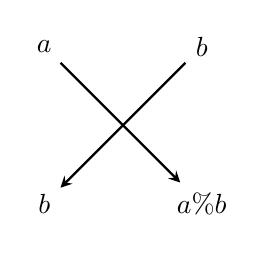
\begin{tikzpicture}[->, thick, >=stealth]

% Nodes
\node (a) at (0,2) {\(a\)};
\node (b) at (2,2) {\(b\)};
\node (mod) at (2,0) {\(a \% b\)};
\node (b2) at (0,0) {\(b\)};

% Arrows
\draw (a) -- (mod);
\draw (b) -- (b2);

\end{tikzpicture}
\end{center}

\begin{python}
# recursive abbr
def gcd(a, b):
    if b == 0:
        return a
        
    return gcd(b, a % b)

# iterative     
def gcd(a, b):
    while b != 0:
        a, b = b, a % b

    return a
\end{python}

\rih{Proof}. Euclidean Algorithm. The Euclidean algorithm is based on the principle that the GCD of two numbers $a$ and $b$ is the same as the GCD of $b$ and $a\%b$ until $b$ becomes zero. Prove the following recursive form:
$$
gcd(a,b) = gcd(b, r)
$$
\begin{enumerate}
\item \rih{Divisibility}: Let $g$ be the GCD of $a$ and $b$. By definition, $g$ divides both $a$ and $b$. From the equation $a=b\cdot q+r$, it follows that $g$ must also divide the remainder $r$, because any divisor of both $a$ and $b$ divides linear combination of them: $r = a - b \cdot q$. 
\item \rih{Reduction}: If we replace $a$ with $b$ and $b$ with $r$, the GCD remains unchanged, and the problem size gets smaller (since $r<b$). 
\item \rih{Termination}: The algorithm repeatedly reduces the size of the numbers by replacing the larger number with the remainder. Eventually, one of the numbers will become zero, and the GCD is the other number, since $gcd(a,0)=a$.
\end{enumerate}
\section{Power}
\runinhead{power(x, n).} To calculate $x^n$. 
\runinhead{Core Clues}:
\begin{enumerate}
\item $O(N)$ is trivial, need to do better than it
\item Divide the problem by half
\begin{align*}
x^n &= (x^2)^{n/2} \\
x^n &= x^{n/2} * x^{n/2} * x^{n \mod 2}
\end{align*}
\end{enumerate}
\begin{python}
def pow(self, x, n):
    is_invert = False if n > 0 else True

    n = abs(n)
    ret = 1.0
    while n > 0:
        if n & 1 == 1:
            ret *= x

        n >>= 1
        x *= x

    if is_invert:
        ret = 1.0 / ret

    return ret
\end{python}
\section{Prime Numbers}
\subsection{Sieve of Eratosthenes}
\subsubsection{Basics}
To find all the prime numbers less than or equal to a given integer n by Eratosthenes' method:
\begin{enumerate}
\item Create a   list of consecutive integers from 2 through n: (2, 3, 4, ..., n).
\item Initially, let $p$ equal 2, the first prime number.
\item Starting from $p$, enumerate its multiples by counting to n in increments of  $p$, and mark them in the list (these will be $2p$, $3p$, $4p$, ... ; the $p$ itself should not be marked).
\item Find the first number greater than $p$ in the list that is not marked. If there was no such number, stop. Otherwise, let $p$ now equal this new number (which is the next prime), and repeat from step 3.
\end{enumerate}

When the algorithm terminates, the numbers remaining not marked in the list are all the primes below $n$.

\subsubsection{Refinements}
The main idea here is that every value for $p$ is prime, because we have already marked all the multiples of the numbers less than $p$. Note that some of the numbers being marked may have already been marked earlier (e.g., 15 will be marked both for 3 and 5).

As a refinement, it is sufficient to mark the numbers in step 3 starting from $p^2$, because all the smaller multiples of $p$ will have already been marked at that point by the previous smaller prime factor other than $p$. From $p^2$, $p$ becomes the smaller prime factor of a composite number. This means that the algorithm is allowed to terminate in step 4 when $p^2$ is greater than n.

For example, consider $p=5$. The first multiple of 5 that we need to mark is $5^2 = 25$, because: 
\begin{enumerate}
\item $5 \times 2 = 10$ has already been marked when processing $p = 2$.
\item $5 \times 3 = 15$ has already been marked when processing $p = 3$ 
\item $5 \times 4 = 20$ has already been marked when processing $p = 2$. 
\end{enumerate}
Therefore, we only need to start marking multiples from $p^2$, since all smaller multiples of $p$ have already been handled.

\begin{python}
def count_primes_sieve(N):
    if N < 2:
        return 0
    # intialize all numbers prime candidates
    primes = [True for _ in range(N+1)]
    # 0 and 1 are not prime numbers
    primes[0] = primes[1] = False

    p = 2
    while (p * p <= N):
        if primes[p]:
            for i in range(p * p, N+1, p):
                primes[i] = False
        p += 1

    return sum(prime)
\end{python}

\rih{Time complexity}. Iterating \pyinline{p} is $O(N)$ and for all the prime number, each inner loop take $\frac{N}{p}$. Then it becomes 

$$
\sum_{p \leq N} \frac{N}{p} = N \sum_{p \leq N} \frac{1}{p}
$$

It looks like $O(N \log N)$ but $p$ are prime numbers, it becomes $O(N \log \log N)$. The \rih{Prime Number Theorem} tells us that the number of primes less than or equal to $N$ is approximate
$$
\frac{N}{\log N}
$$


Another refinement is to initialize list odd numbers only, (3, 5, ..., n), and count in increments of $2p$ in step 3, thus marking only odd multiples of $p$. This actually appears in the original algorithm. This can be generalized with wheel factorization, forming the initial list only from numbers coprime with the first few primes and not just from odds (i.e., numbers coprime with 2), and counting in the correspondingly adjusted increments so that only such multiples of $p$ are generated that are coprime with those small primes, in the first place.



To summarized, the refinements include:
\begin{enumerate}
\item Starting from $p^2$; thus $p$ is the smaller prime factor. 
\item Preprocessing even numbers and then only process odd numbers; thus the increment becomes $2p$.
\end{enumerate}

\begin{python}
def count_primes(N):
    if N < 3:
        return 0
    primes = [
        False if i%2 == 0 else True 
        for i in range(n)
    ]
    primes[0], primes[1] = False, False
    for i in range(3, int(math.sqrt(N))+1, 2):
        if primes[i]:
            for j in range(i*i, n, 2*i):
                primes[j] = False

    return prime.count(True)
\end{python}

\subsection{Factorization}
Backtracking: Section-\ref{factorization}.

\section{Median}
\subsection{Basic DualHeap}
\runinhead{Sliding Window Median.} Find the list of median in the sliding window. $\Ra$ Dual heap with lazy deletion.

DualHeap to keep track the median when a method to find median is called multiple times.

Here we use the negation of the value as a trick to convert min-heap to max-heap.
\begin{python}
import heapq

class DualHeap:
  def __init__(self):
    self.min_h = []
    self.max_h = []  # need to negate the value 

  def insert(self, num):
    if not self.min_h or num > self.min_h[0]:
      heapq.heappush(self.min_h, num)
    else:
      heapq.heappush(self.max_h, -num)
    self.balance()

  def balance(self):
    l1 = len(self.min_h)
    l2 = len(self.max_h)
    if l1-l2 > 1:
      heapq.heappush(self.max_h, 
                     -heapq.heappop(self.min_h))
      self.balance()
    elif l2-l1 > 1:
      heapq.heappush(self.min_h, 
                     -heapq.heappop(self.max_h))
      self.balance()
    return

  def get_median(self):
    """Straightforward"""
\end{python}

\subsection{DualHeap with Lazy Deletion}\label{dh_lazy_del}
Clues:
\begin{enumerate}
\item Wrap the value and wrap the heap
\item When delete a value, mark it with tombstone. 
\item When negate the value, only change the value, not the reference. 
\item When heap pop, clean the op first. 
\end{enumerate}
\begin{python}
import heapq
from collections import defaultdict
from dataclasses import dataclass

@dataclass
class Value:
    val: int
    deleted: bool


class Heap:
    def __init__(self):
        self.h = []
        self.len = 0

    def push(self, item):
        heapq.heappush(self.h, item)
        self.len += 1

    def pop(self):
        self._clean_top()
        self.len -= 1
        return heapq.heappop(self.h)

    def remove(self, item):
        """lazy delete"""
        item.deleted = True
        self.len -= 1

    def __len__(self):
        return self.len

    def _clean_top(self):
        while self.h and self.h[0].deleted:
            heapq.heappop(self.h)

    def peek(self):
        self._clean_top()
        return self.h[0]


class DualHeap:
    def __init__(self):
        self.min_h = Heap()  # represent right side
        self.max_h = Heap()  # represent left side
    # others similar as the previous section's above DualHeap
\end{python}

\section{Modular}
\subsection{Power of 4}
To check whether a number of the power of 4, we can check whether it mod 3 equals 1.
\begin{align*}
4^a &\equiv 1^a\mod 3 \\
&\equiv 1 \mod 3
\end{align*}

Alternatively, we can use bit manipulation based on the power of 4 in the binary form of \pyinline{repeat n 1 << 2}, and checks whether there is even number of 0's in binary form. 

\section{Ord}
\runinhead{Number in lexical order.} Given an integer n, return 1 ~ n in lexicographical order. For example, given 13, return: [1,10,11,12,13,2,3,4,5,6,7,8,9].

Enumerate to find the pattern:
\begin{python}
1	10	11	...	19
2	21	22	...	29
3	31	32	...	39
4 ...
.
.
\end{python}

Using DFS.
\begin{python}
def dfs(cur, ret, N):
    ret.append(cur)
    for d in range(10):
        nxt = cur * 10 + d
        if nxt <= N:
            dfs(nxt, ret, N)
        else:
            break

N = 105
ret = []
for i in range(1, 10):
    if i <= N:
        dfs(i, ret, N)
    else:
        break
\end{python}

Optionally, using iterative appraoch. 
\begin{python}
def gen():
    i = 1
    for _ in range(n):
        yield i
        if i * 10 <= n:
            i *= 10  # * 10
        elif i % 10 != 9 and i + 1 <= n:
            i += 1  # for current digit
        else:
            while i % 10 == 9 or i + 1 > n:
                i //= 10
            i += 1
\end{python}

\chapter{Bit Manipulation}

\section{Introduction}
Queue, Stack

\chapter{Greedy}

\section{Introduction}
Philosophy: choose the best options at the current state without reverting the choice in the future. 

A greedy algorithm is an algorithm that follows the problem solving heuristic of making the locally optimal choice at each stage with the hope of finding a global optimum.

% !TEX root = algo-quicksheet.tex
\chapter{String}

\section{Palindrome}
\subsection{Palindrome anagram}
\begin{itemize}
\item \rih{Test palindrome anagram.} Char counter, number of odd count should $\leq 0$.
\item \rih{Count palindrome anagram.} See Section-\ref{N_objects_K_types}.
\item \rih{Construct palindrome anagram.} Construct all palindrome anagrams given a string \pyinline{s}.
\end{itemize}

\runinhead{Core Clues:}
\begin{enumerate}
\item Different choices of char $\Ra$ backtracking, choose the next from the char counters of \pyinline{s}. 
\item To avoid loop $\Ra$ jump parent char
\end{enumerate}

\begin{python}
def backtrack(self, s, counters, pi, cur, ret):
  if len(cur) == len(s):
    ret.append(cur)
    return

  for k in counters.keys():
    # jump the parent
    if k != pi and counters[k] > 0:
      for n in range(1, counters[k]/2+1):
        counters[k] -= n*2
        self.backtrack(s, counters, k, k*n+cur+k*n, ret)
        counters[k] += n*2
\end{python}

Jump within the iterations of choice to avoid dead loop. 

How to handle odd counter? Check outside the backtrack, and potentially raise error. 

\subsection{Number}
\runinhead{Next Permutation.} Given a string $n$ representing an int, return the closest int (not including itself), which is a palindrome. For example $n = `123'$, return $`121'$. 

\begin{enumerate}
\item Palindrome $\Ra$ Mirror the left half of $n$.
\item 19997 has two candidates 19991 and 20002 $\Ra$ for the half, $+/-1$ for carry/borrow
\item 1000 has two candidates 999 and 1001 $\Ra$ More/less digits of $n$ $\Ra$ checking numbers $10..0, 9..9$
\end{enumerate}
\begin{python}
def nearestPalindromic(self, s: str) -> str:
  l = len(s)
  odd_l = l & 1
  if odd_l:
    half = s[:l//2] + s[l//2]
  else:
    half = s[:l//2]

  def mir(half: str) -> str:
    if not odd_l:
      return half + half[::-1]
    else:
      return half + half[::-1][1:]

  # candidates
  cands = {
    mir(str(int(half) - 1)), 
    mir(half), 
    mir(str(int(half) + 1)),
  }
  cands |= {
    str(10 ** l + 1), 
    str(10 ** (l - 1) - 1)
  }
  cands.discard(s)
  return min(
    cands, 
    key=lambda e: (abs(int(s) - int(e)), int(e))
  )
\end{python}
\section{Anagram}
\runinhead{Group of strings by anagram.}

Using a frequency vector 
\begin{python}
class Solution:
  def groupAnagrams(self, strs):
    # key: 26-tuple counts; value: list of words
    d = defaultdict(list)
    for s in strs:
      cnt = [0] * 26
      for ch in s:
        cnt[ord(ch) - ord('a')] += 1
      d[tuple(cnt)].append(s)
    return list(d.values())
\end{python}

\section{KMP}
Find the pattern $p$ in string $s$ within complexity of $O(|P|+|S|)$.

\subsection{Prefix matching suffix table}
Intuition: when a mismatch happens at $p_i$ vs $s_i$, don't restart from $p_0$; instead jump to the next best candidate $i$ right after the matched prefix \& suffix, keeping the already verified prefix.

Let $L_i$ be the length of the longest proper prefix that matches a suffix ending at $p_i$. 
\begin{enumerate}
\item A proper prefix is a prefix that is not equal to the whole string itself. Proper ensures that $L_i < i+1$.
\item Need to maintain the longest proper prefix of a substring that is also a suffix of it.
\end{enumerate}

\begin{table}[h!]
\centering
\begin{tabular}{c|ccccccc}
  \toprule
  \textbf{i}   & 0 & 1 & 2 & 3 & 4 & 5 & 6 \\
  \midrule
  \textbf{$p_i$} & A & B & C & D & A & B & D \\
  \textbf{$L_i$} & 0 & 0 & 0 & 0 & 1 & 2 & 0 \\
  \bottomrule
\end{tabular}
\end{table}
\begin{python}
def kmp_lps(p):
    L = [0] * len(p)
    i = 1
    pre = 0
    while i < len(p):
        if p[i] == p[pre]:
            L[i] = pre + 1
            pre += 1
            i += 1
        elif pre:  # fallback
            pre = L[pre - 1]
        else:  # no fallback
            L[i] = 0
            i += 1

    return L
\end{python}
Time complexity:
\begin{itemize}
\item From code itself it appears to be $O(|P|^2)$.
\item Define $\Delta = i - pre$.
\item $i$ never goes backward - $i$ either forwards of stays.
\item Any time $i$ doesn’t move forward, $\Delta$ must rise
\item $j$ is bounded by $O(|P|)$ and $\Delta$ is bounded by $O(|P|)$
\end{itemize}
\subsection{Searching algorithm}
\begin{figure}[]
\centering
\subfloat{\includegraphics[width=0.8\linewidth]{kmp_presuffix}}
\caption{KMP example}
\label{fig:kmp_presuffix}
\end{figure}


\begin{python}
def kmp_search(p, s):
    L = kmp_lps(p)
    ret = []
    i = 0
    j = 0
    while j < len(s):
        if p[i] == s[j]:
            i += 1
            j += 1
            if i == len(p):
                ret.append(j - i)
                i = L[i - 1]
        elif i:
            i = L[i - 1]
        else:
            j += 1

    return ret
\end{python}
Time compelxity:
\begin{itemize}
\item Define $\Delta = j - i$.
\item $j$ never goes backward
\item Any time $j$ doesn’t move forward, $\Delta$ must rise
\item $j$ is bounded by $O(|S|)$ and $\Delta$ is bounded by $O(|P|+|S|)$
\end{itemize}
\subsection{Applications}
\begin{enumerate}
\item Find needle in haystack. 
\item Shortest palindrome 
\end{enumerate}
\subsection{Subsequence}
Given a string $s$ and an array of strings $words$, return the number of $words_i$ that is a subsequence of $s$. For example, input: \pyinline{s = "abcde"}, \pyinline{words = ["a","bb","acd","ace"]}

\rih{Core clues:}
\begin{enumerate}
\item Test whether one string is another's subsequence is straightforwad, how to test multiple strings is one's subsequence? $\Ra$ consume the multiple strings in one iteartion. 
\item Each character can be a candidate $\Ra$ char map. 
\item Each $words_i$ is only match once $\Ra$ iterator 
\end{enumerate}
\begin{python}
def numMatchingSubseq(self, S, words) -> int:
  """
  Linear O(|S| + sum(|word|)) 
  no need to if-check with HashMap + Iterator 
  """ 
  itr_lsts = defaultdict(list) 
  for w in words: 
    itr_lsts[w[0]].append(iter(w[1:])) 

  for c in S: 
    itrs = itr_lsts.pop(c, []) 
    for itr in itrs: 
      ch = next(itr, None) 
      itr_lsts[ch].append(itr) 
  
  return len(itr_lsts[None])
\end{python}
Note \pyinline{itr_lsts} can be short formed as \pyinline{itrss}


\chapter{Graph}


\section{TOPOLOGICAL SORTING}
For a graph $G=\{V, E\}$, $ A \rightarrow B $, then $A$ is before $B$ in the ordered list. 
\subsection{Algorithm}
General algorithm and notice.\\
 
dfs:
\begin{enumerate}
\item \textbf{Dfs neighbors first}. If the neighbors of current node is  $\neg$visited, then dfs the neighbors
\item \textbf{Dfs current node}. After visiting all the neighbors, then visit the current node and push it to the result queue.
\item \textbf{Reverse}. Reverse the result queue. 
\end{enumerate}

Notice:
\begin{enumerate}
\item Need to reverse the result queue, since the neighbors (successors) are visited first. 
\item Need to detect cycle; thus the dfs need to construct result queue and detect cycle simultaneously, by using two sets: $visited$ and $marked$. 
\end{enumerate}

\subsection{Code}
\begin{lstlisting}[language=python]
def topological_sort(self, V):
    visited = set()
    marked = set()
    ret = []

    for k in V.keys():
        if k not in visited:
            if not self.dfs(V, k, visited, marked, ret):
                return []

    ret.reverse()
    return ret

def dfs(self, V, k, visited, marked, ret):
    if k in marked:
        return False

    marked.add(k)
    for neighbor in V[k]:
        if neighbor not in visited:
            if not self.dfs(V, neighbor, visited, marked, ret):
                return False

    marked.remove(k)
    visited.add(k)
    ret.append(k)
    return True
\end{lstlisting}

\subsection{Applications}
\begin{enumerate}
\item Course scheduling problem with pre-requisite. 
\end{enumerate}


\chapter{Interval}


\section{Introduction}
\rih{Two-way range.} The current scanning node as the pivot, need to scan its left neighbors and right neighbors. 
$$
|\leftarrow p \rightarrow |
$$

If the relationship between the pivot and its neighbors is symmetric, since scanning range is $[i-k, i+k]$ and iterating from left to right, only consider $[i-k, i]$ to avoid duplication.
$$
|\leftarrow p
$$


% !TEX root = algo-quicksheet.tex
\chapter{Dynamic Programming}



\section{Introduction}
The philosophy of dp:
\begin{enumerate}
\item The definition of \textbf{states}: redefine the original problem into relaxed substructure. 
\item The definition of the \textbf{transition functions} among states 
\end{enumerate} 

The so called concept dp as memoization of recursion does not grasp the core philosophy of dp. 

The formula in the following section are unimportant. Instead, what is important is the definition of dp array and transition function derivation.

\runinhead{State definitions.} The state definition is the \textbf{redefinition} of the original problem as substructure. 

Three general sets of state definitions of the substructure. 
\begin{enumerate}
\item ends \textit{at} index $i$ ($i$ \textbf{required})
\item ends \textit{before} index $i$ ($i$ \textbf{excluded})
\item ends \textit{at} or \textit{before} i.e. \textit{up to} index $i$ ($i$ \textbf{optional})
\end{enumerate}
\subsection{Common programming practice}
\runinhead{Dummy.} Use dummies to avoid using if-else conditional branch.
\begin{enumerate}
\item Use $n+1$ dp arrays to reserve space for dummies. 
\item Iteration range is $[1, n+1)$.
\item $n+k$ for k dummies  
\end{enumerate}


\runinhead{Space optimization - collapsed state.} To avoid MLE, we need to carry out space optimization. Let $o$ be other subscripts, $f$ be the transition function. 

Firstly,
$$
F_{i, o} = f\big(F_{i-1, o'}\big)
$$

should be reduced to 
$$
F_{o} = f\big(F_{o'}\big)
$$

Secondly,
$$
F_{i, o} = f\big(F_{i-1, o'}, F_{i-2. o'}\big)
$$

should be reduced to 
$$
F_{i, o} = f\big(F_{(i-1)\%2, o'}, F_{(i-2)\%2. o'}\big)
$$

More generally, we can be $(i-b)\%a$ to reduce the space down to $a$.

Notice:
\begin{itemize}
\item $F_{i, o}$ depends on $F_{i-1, o} \Ra$ must iterate $i$ \textbf{backward} to un-updated value. 
\end{itemize}

\runinhead{Backtrace array.} Normally dp returns the number of count/combinations. To reconstruct the result, store the parent index a backtrace array . 

$$
\pi[i]=j
$$


\section{Sequence}\label{dpSequence}
\subsection{Best Trailing Subarrays - Kadane's Algorithm}
Kadane’s algorithm tracks the \textit{best} subarray ending AT each position.

\runinhead{Maximum Subarray Sum.} Find the maximum subarray sum of $A$.  

Let $F_i$  be the maximum subarray sum ending at $A_{i}$
$$
F_i = \max(F_{i-1}+A_{i}, 0)
$$

Then the global $maxa$ is:
$$
maxa = \max(F_i\cdot \forall i)
$$

We can do index rewrite - let $F_i$ be the max subarray sum for $A[:i]$ up to $A_{i-1}$.
$$
F_i = \max(F_{i-1}+A_{i-1}, 0)
$$

\runinhead{Number of 1s-subarrays (1D).} Find the total number of 1s-subarrays. For example, for $A = [1, 0, 1, 1, 1]$, there are $7=1+1+2+3$ 1s-subarrays. 

Let $F_j$ be number of 1s-subarrays ending AT $j-1$:
\[
F_j = 
\begin{cases}
   F_{j-1} + 1 & \text{if } A_{j-1} = 1, \\
   0 & \text{otherwise}.
\end{cases}
\]
The total number of 1s-subarrays is $\sum{F}$.

\runinhead{Number of 1s-submatrix (2D).} For a 2-D matrix, find the total number of 1s-submatrices. Consider a 2-row matrix:
$$
\left[\begin{array}{ccccc}
1 & 0 & 1 & 1 & 1 \\
1 & 1 & 0 & 1 & 1
\end{array}\right]
$$
Project 2D into 1D:
$$
\left[\begin{array}{ccccc}
1 & 0 & 0 & 1 & 1 
\end{array}\right]
$$

\[
F_j = 
\begin{cases}
   F_{j-1} + 1 & \text{if } M_{lo:hi,j-1} = 1, \\
   0 & \text{otherwise}.
\end{cases}
\]


\begin{python}
def num_submat(mat):
    ret = 0
    M = len(mat)
    N = len(mat[0])
    for lo in range(M):
        # is all ones for mat[lo:hi][j]
        is_ones_col = [True for j in range(N)] 
        for hi in range(lo+1, M+1):
            for j in range(N):
                is_ones_col[j] &= mat[hi-1][j]
                # mem saving

            F = [0 for _ in range(N+1)]
            for j in range(1, N+1):
                F[j] = F[j-1] + 1 if is_ones_col[j-1] \
                       else 0 
                ret += F[j]
    
    return ret
\end{python}

\runinhead{Maximum Subarray Gain.} Find the maximum subarray gain of $A$. A gain is defined as followed:
\[
gain(A_i) = 
\begin{cases}
  +1 & \text{if } A_i = t, \\
  -1 & \text{if } A_i = k, \\
   0 & \text{otherwise}.
\end{cases}
\]


Let $F_i$  be the maximum subarray gain ending at $A_{i}$
$$
F_i = \max\Big(F_{i-1}+gain(A_{i}), 0\Big)
$$
\subsection{Single-state dp}
\runinhead{Longest common subsequence (LCS).} Let $F_{i, j}$ be the LCS at string $A[:i+1]$ and $B[:j+1]$, up to $A_i$ and $B_j$. Note subsequence does not have to be continuous. 

We have two situations: $A_i=B_j$ or not.

\[
F_{i, j} = 
\begin{cases}
  F_{i-1, j-1}+1 & \text{if } A_i=B_j, \\
  \max\Big(F_{i-1, j}, F_{i,j-1}\Big) & \text{otherwise}.
\end{cases}
\]
No need to set 0 since it is subsequence. 
\begin{center}
\begin{tikzpicture}[
    scale=1.5,
    every node/.style={draw, minimum size=1cm},
    ->, >=Stealth
  ]
  % Draw nodes
  \node (A) at (0,1) {};
  \node (B) at (1,1) {};
  \node (C) at (0,0) {};
  \node (D) at (1,0) {};

  % Draw arrows
  \draw[->, ultra thick] (A) -- (D);
  \draw[->, thick] (B) -- (D);
  \draw[->, thick] (C) -- (D);
\end{tikzpicture}
\end{center}

\begin{python}
def lcs_edit(A, B):
    """Return (=, -, +) git diff via classic LCS."""
    M, N = len(A), len(B)
    F = [
        [0]*(M+1) 
        for _ in range(N+1)
    ]
    for i in range(M):
        for j in range(N):
            if A[i] == B[j]:
                F[i+1][j+1] = F[i][j] + 1  
            else:
                F[i+1][j+1] = max(F[i][j+1], F[i+1][j])
\end{python}

To reconstruct the edits of `+/-/=' with $A$ as the base string:
\begin{enumerate}
\item Forward reconstruct? Greedy? $aa\alpha\beta b$ vs. $ab\gamma \delta c$, cannot decide by looking ahead by 1 position; thus become a search problem
\item Instead backward reconstruct since $F_{i, j}$ is defined up to $A_i, B_j$.
\end{enumerate}
\begin{python}
def reconstruct(A, B, F):
    M, N = len(A), len(B)
    ret = []
    # backward pass
    i, j = M, N
    while i or j:
        if i and j and A[i-1] == B[j-1]:
            ret.append(("=", a[i-1]))
            i -= 1
            j -= 1
        elif j and (i == 0 or F[i][j-1] >= F[i-1][j]):
            # B[:j-1] has longer LCS than A[:i-1]
            ret.append(("+", B[j-1]))
            j -= 1
        else:
            ret.append(("-", A[i-1]))
            i -= 1
    ret.reverse()
    return ret
\end{python}
\runinhead{Longest common substring.} Let $F_{i, j}$ be the LCS at string $a[:i]$ and
$b[:j]$. We have two situations: $a[i]=b[j]$ or not.
\[
F_{i, j} = 
\begin{cases}
  F_{i-1, j-1}+1 & \text{if } a[i]=b[j], \\
  0 & \text{otherwise}.
\end{cases}
\]


Because it is not necessary that $F_{i,j}\geq F_{i',j'}, \forall i,j\cdot i>i', j>j'$, as $F_{i,j}$ can be 0, thus  $gmax=\max\big(F\big)$.
\runinhead{Longest increasing subsequence (LIS).} Find the longest increasing subsequence of an array $A$.

let $F_i$ be the LIS length ends at $A_i$. 
\begin{eqnarray*}
F_i = \max(F_j+1, \forall j < i \cdot A_j<A_i)
\end{eqnarray*}

Then the global $maxa$ is:
$$
maxa = \max(F_i\cdot \forall i)
$$

Time complexity: $O(n^2)$

How to improve time complexity? 

Notice that $F_i$ is taking $\max$ over previous $F_j$, which makes $F_i > F_j$, although $F$ as a whole is not monotonic increasing. 

To binary search to achieve $O(n \log n)$, we need to maintain monotonic states. $F$ records length, can we do the inverse - $V_i$ records some element/value of the LIS of some length $i$.

Let $V_{j}$ be the smallest tail value of the LIS of length $j+1$. 
$$
V_j = \arg\min_k\{ F_k = j+1, \forall k < j\}
$$

$V$ is monotonic increasing, maintaining those minima is just monotone queue optimization of recurrence of $F$'s formula.

\rih{Core Clues:}
\begin{enumerate}
\item \pyinline{V}: $V_j$ = min possible tail value of a subseq length $j+1$
\item \pyinline{idx}: Index where each tail value is (index in $A$)
\item \pyinline{pi}: predecessor indices for reconstruction
\end{enumerate}

\begin{python}
def lis(A):
    V = []
    pi = [-1 for _ in A]  # defaultdict(lambda: -1)
    for i in range(len(A)):
        j = bisect.bisect_left(V, A[i], 
            key=lambda e: A[e])

        if j < len(L):
            V[j] = i
        else:
            V.append(i)
        
        pi[i] = V[j-1] if j > 0 else -1

    # rebuild
    ret = []
    cur = V[~0]
    while cur != -1:
        ret.append(A[cur])
        cur = pi[cur]
        
    return ret[::-1]

print(lis([10,9,2,5,3,7,101,18]))   # -> [2, 3, 7, 18]
\end{python}

Ref search section \ref{extremeValueProblem}.

\runinhead{Maximum sum of non-adjacent cells.} Get the maximum sum of non-adjacent
cells of an array $A$.

Let $F_i$ be the maximum sum of non-adjacent cells for $A[:i]$, up to $A_{i-1}$. You have tow options:
choose $A_{i-1}$ or not.
\begin{align*}
F_{i} = \max\big(
&F_{i-1}, \\ 
&F_{i-2}+A_{i-1}
\big)
\end{align*}

\runinhead{Edit distance} Find the minimum number of steps required to convert words $A$ to $B$ using inserting, deleting, replacing. 

Let $F_{i, j}$ be the minimum number of steps required to convert $A[:i]$ to $B[:j]$.
\begin{center}
\begin{tikzpicture}[
    scale=1.5,
    every node/.style={draw, minimum size=1cm},
    ->, >=Stealth
  ]
  % Draw nodes
  \node (A) at (0,1) {};
  \node (B) at (1,1) {};
  \node (C) at (0,0) {};
  \node (D) at (1,0) {};

  % Draw arrows
  \draw[->, thick] (A) -- (D);
  \draw[->, thick] (B) -- (D);
  \draw[->, thick] (C) -- (D);
\end{tikzpicture}
\end{center}
\[
    F_{i, j} =
    \begin{cases}
        F_{i-1, j-1} & \text{if } a[i] = b[j] \\[8pt]
        \min \Big( 
        F_{i, j-1} + 1 & \text{if insert} \\ 
        F_{i-1, j} + 1 & \text{if delete} \\ 
        F_{i-1, j-1} + 1 \Big) & \text{if replace}
    \end{cases}
\]

\runinhead{H-index} Given an array of citations $A$ of a researcher, write a function to compute the researcher's h-index. Find the highest number $h$ such that the researcher has at least $h$ publications that have each been cited at least $h$ times.

Need some re-representation of information: 
\begin{enumerate}
\item Relax the problem $\Ra$ exact $i$ citations: let $C_i$ be the \#paper with $=i$ citations.
\item The original problem $\Ra \geq i$ citations: let $F_i$ be the \#paper with $\geq i$ citations.
\end{enumerate}
$$
F_i = F_{i+1} + C_i
$$

Backward DP. DP takes $O(n)$. 
\begin{python}
def hIndex(A):
    N = len(A)
    C = [0 for _ in range(N+1)]
    for e in A:
        C[min(e, N)] += 1

    F = [0 for _ in range(N+2)]
    for i in range(N, -1, -1):
        F[i] += F[i+1] + C[i]
        if F[i] >= i:
            return i

    return 0
\end{python}

Given $F_i > F_{i+1}$, as $F$ is sorted, use binary search to achieve $O(\lg n)$.

\runinhead{Interleaving String} Given $s, a, b$ find whether $s$ is formed by the interleaving
of $a$ and $b$.

Let $F_{i,j}$ be \pyinline{s[:i+j]} is interleaved from \pyinline{a[:i], b[:j]}, a boolean.

We have to options to choose \pyinline{s[i+j-1]}, either from \pyinline{a[i-1]} or from \pyinline{b[j-1]}:
\begin{align*}
F_{i,j} = &\Big(F_{i-1, j} \wedge s_{i+j-1} = a_{i-1}\Big) \\
 \vee &\Big(F_{i,j-1} \wedge s_{i+j-1} = b_{j-1}\Big)
\end{align*}

\runinhead{Largest divisible subset.} Given a list of distinct positive integers $A$, find the largest subset $S$ such that every pair $(S_i, S_j)$ of elements in this
subset satisfies: $S_i \% S_j = 0 \text{ or } S_j \% S_i = 0$.

Let $F_i$ be the length of the divisible subset ending at $A_i$. 

$$
F_i = \max_{j: j< i, A_i\%A_j=0}(1+F_j)
$$

Let $\pi_i$ be the index of the previous element of $A_i$ in the divisible subset. $\pi_i$ is used to reconstruct the array.

$$
\pi_i = \arg\max_{j: j< i, A_i\%A_j=0}(1+F_j)
$$
\runinhead{Maximum Earnings From Taxi.} Given $n$, representing driving from point 1 to point n to make money by picking up passengers. Given $rides$, representing i-th passenger ride from point $start_i$ to point $end_i$ who is willing to give a $tip_i$ dollar tip. The reward is $tip_i + end_i - start_i$. Find the maximal reward. 

\rih{Core clues:}
\begin{enumerate}
\item Going from 1 to $n$ $\Ra$ sort the passengers by $start$ or $end$ $\Ra$ sort through a dict
\item Need to consider vacant $\Ra$ $F_i = max(F_i, F_{i-1})$.
\item One pass from 1 to $n$
\end{enumerate}
Look-back DP.

Let $F_i$ be the max reward at point $i$
$$
F_i = \max\Big(F_{i-1}, F_j + (tip_j + i - j)\cdot \forall j\Big)
$$
\begin{python}
def maxTaxiEarnings(self, n, rides):
  ends = defaultdict(list)
  for s, e, tip in rides:
    ends[e].append((s, tip))

  F = [0 for _ in range(n+1)]

  for i in range(1, n + 1):
    F[i] = max(F[i], F[i-1])
    if i in ends:
      for s, tip in ends[i]:
        F[i] = max(F[i], F[j] + tip + i - s)

  return F[n]
\end{python}

Look-ahead DP.


\begin{python}
def maxTaxiEarnings(self, n, rides):
  starts = defaultdict(list)
  for s, e, tip in rides:
    starts[s].append((e, tip))

  F = [0 for _ in range(n + 1)]

  for i in range(1, n + 1):
    F[i] = max(F[i], F[i-1])
    if i in starts:
      for e, tip in starts[i]:
        F[e] = max(F[e], F[i] + tip + e - i)

  return F[n]
\end{python}




\subsection{Dual-state dp}
\runinhead{Maximal product subarray.} Find the subarray within an array $A$ which has the largest product. 
\begin{itemize}
\item Maximal product $\Ra$ Let $L_i$ be the largest product end at $A_i$.
\item Product can be negative $\Ra$ Let $S_i$ be the smallest product end at $A_i$. 
\item The states can be negative. 
\end{itemize}
\begin{eqnarray*}
&& S_i = \min\Big( A_i,\ S_{i-1}\cdot A_i,\ L_{i-1}\cdot A_i \Big)
\nonumber \\
&& L_i = \max\Big( A_i,\ S_{i-1}\cdot A_i,\ L_{i-1}\cdot A_i \Big)
\end{eqnarray*}

It can be optimized to use space $O(1)$. 

\runinhead{Trapping Rain Water}
Given $n$ non-negative integers representing an elevation map where the width of each
bar is 1, compute how much water it is able to trap after raining.
\begin{figure}[]
    \centerline{\includegraphics[height = 1in]{rainwatertrap}}
    \caption{Trapping Rain Water}
  \label{fig:rainwatertrap}
\end{figure}

Let $L_i$ be the $\max(A[:i])$; let $R_i$ be the $\max(A[i:])$. The dp of obtaining $L, R$ is trivial. 

The the total volume $vol$:
$$
vol = \sum_i\max\big(0,\min(L_i, R_{i+1})-A[i]\big)
$$
\runinhead{Zigzag subsequence.} Find the max length zigzag subsequence which goes up and down alternately within the array $A$.

Let $U_i$ be the max length of zigzag subsequence end at $A_i \wedge$ going up.

Let $D_i$ be the max length of zigzag subsequence end at $A_i \wedge$ going down.
\begin{align*}
U_i &= \max(D_j+1 \cdot \forall j < i \cdot \text{ if $A_i > A_j$})  \\ 
D_i &= \max(U_j+1 \cdot \forall j < i \cdot \text{ if $A_i < A_j$})  
\end{align*}

Notice in python implementation, the two states are interleaved and interdependent. 
\begin{python}
def maxzigzag(self, A):
    N = len(A)
    U = [1 for _ in range(N)]
    D = [1 for _ in range(N)]
    gmax = 1
    for i in range(1, N):
        for j in range(i):
            if A[i] > A[j]:
                U[i] = max(U[i], D[j] + 1)
            elif A[i] < A[j]:
                D[i] = max(D[i], L[j] + 1)

            gmax = max(gmax, U[i], D[i])

    return gmax
\end{python}
Greedy compression. Let $D_i$ be the length of longest zigzag subsequence up to $A_I$, with last step downward. 
\[
D_i =
  \begin{cases}
   U_{i-1} + 1 &\text{if } A_{i} < A_{i-1}  \\
   D_{i-1} & \text{otherwise}
\end{cases}
\]

For $D_i$, we only need to check $A_{i-1} > A_{i}$ since otherwis $A_{i-3}, A_{i-2}, A_{i-1}...$ keeps going up.

\[
H_i =
  \begin{cases}
   H_{i-1} &\text{if upward trend continues}  \\
   D_{i-1} + 1 &\text{otherwise, i.e. } A_i > A_{i-1}
\end{cases}
\]
Note that 
$$
|H_i - D_i| \leq 1 \cdot \forall i
$$
\begin{center}
\begin{tikzpicture}[->, >=stealth', auto, node distance=2cm, semithick]

  % States
  \node[state] (H) {H};
  \node[state, below of=H] (D) {D};

  % Self-loops
  \path (H) edge[loop above] (H);
  \path (D) edge[loop below] (D);

  % Transitions between H and D
  \path (H) edge[bend left=25] (D);
  \path (D) edge[bend left=25] (H);

\end{tikzpicture}

\begin{tikzpicture}[
    ->, >=Stealth, semithick,
    neuron/.style={circle, draw, minimum size=18pt, inner sep=0pt}
]

%--- neurons ---
\node[neuron] (Hi_1) at (0, 1.2) {$H_{i-1}$};
\node[neuron] (Di_1) at (0,-1.2) {$D_{i-1}$};

\node[neuron] (Hi)   at (3, 1.2) {$H_i$};
\node[neuron] (Di)   at (3,-1.2) {$D_i$};

%--- connections (fully connected 2x2) ---
\draw (Hi_1) -- (Hi);   % H_{i-1} -> H_i
\draw (Hi_1) -- (Di);   % H_{i-1} -> D_i
\draw (Di_1) -- (Hi);   % D_{i-1} -> H_i
\draw (Di_1) -- (Di);   % D_{i-1} -> D_i
\end{tikzpicture}
\end{center}

\begin{python}
def maxzigzag(self, A):
    N = len(A)
    U = [1 for _ in range(N)]
    D = [1 for _ in range(N)]
    for i in range(1, N):
        D[i] = U[i-1] + 1 if A[i] < A[i-1] else D[i-1]
        U[i] = D[i-1] + 1 if A[i] > A[i-1] else U[i-1]

    return max(U[N-1], D[N-1])
\end{python}
\runinhead{Buy low sell high.} Given a stock price timeseries $A$, find the maximum profit, with at most $k$ transactions.
Let $L_{i,j}$ be the global max ending at $A_i$ with $j$ transactions. Let $G_{i,j}$ be the global max ending at or before (i.e. up to) $A_i$ with $j$ transactions. Kadance-style.
\begin{align*}
\Delta &= A_i - A_{i-1} \\ 
L_{i,j} &= \max(G_{i-1,j-1}+\Delta, L_{i-1,j}+\Delta) \\
G_{i,j} &= \max(L_{i, j}, G_{i-1,j}) 
\end{align*}
\begin{python}
def dp(A, k):
    n = len(A)
    L = [0 for _ in range(k+1)]  # local max
    G = [0 for _ in range(k+1)]  # global max
    ret = 0
    for i in range(1, n):
        delta = A[i] - A[i-1]
        for j in range(k, 0, -1):
            L[j] = max(G[j-1] + delta, L[j] + delta)
            G[j] = max(L[j], G[j])
            ret = max(ret, G[j])

    return ret
\end{python}
\subsection{Synchronized States}
\runinhead{Cherry pickup.} Given a $n \times n$ matrix $M$, 0 is a pass through block, 1 is a reward, -1 is block. Find the maximum reward going from $(0, 0)$ to $(\sim 0, \sim 0)$ and then back to $(0, 0)$. 

\rih{Core clues:}
\begin{enumerate}
\item If the problem is relaxed to two passes in two parallel matrics, it is trivial. However, the reward can only take once. Thus union the reward, not add the rewards. 
\item In forward path, we take $k$ steps from the start. In backward path, we take $k$ steps to reach the start. 
\item Equivalently, from start to end and then back to start $\Ra$ treat them as start to end twice
\end{enumerate}
The basic transition for one pass
$$
F_{i,j} = \max(F_{i, j}, F_{i-1, j}, F_{i, j-1})
$$
Given $k$, we can use $i$ to determine $j$ as \fbox{$i+j=k$}. We only need to know the forward pass row index $i$ and backward $i'$. 

\begin{align*}
J_{i, i', k} &= \max(J_{i, i', k-1}, J_{i-1, i', k-1}, \\
& J_{i, i'-1, k-1}, J_{i-1, i'-1, k-1}) \\ 
& + reward(M_{i, j}, M_{i', j'})
\end{align*}
The $reward$ function is 
\[
reward(M_{i,j}, M_{i', j'}) = 
\begin{cases}
-\infty &\text{if } M_{i, j} = -1 \lor M_{i', j'} = -1 \\ 
M_{i, j} + M_{i', j'} &\text{if } i \neq i' \\ 
M_{i, j} &\text{if } i = i'
\end{cases}
\]
\subsection{Automata}
\runinhead{Decode ways.} `A' encodes 1, `B' 2, ..., `Z' 26, Given an encoded message containing digits $S$, determine the total number of ways to decode it.

For example, given encoded message 12, it could be decoded as ``AB'' (1 2) or ``L'' (12). Thus, the number of ways decoding 12 is 2.

Let $F_i$ be number of decode ways for $s[:i]$, end at $s[i-1]$. 

\begin{itemize}
\item If $s_{i-1}$ is 0, we only have one way to decode: $10$ or $20$.
$$
F_i = F_{i-2}
$$ 
\item If $s_{i-1}$ is not 0, we have two one ways to decode: 1) $1 \sim 9$; or 2) $10 \sim26$
$$
F_i = F_{i-1}+F_{i-2}
$$
\end{itemize}
\begin{python}
if s[i-1] == "0":
    if s[i-2] in ("1", "2"):
        F[i] = F[i-2]
    else:
        return 0
else:
    F[i] = F[i-1]
    # s[i-2:i]
    if 10 <= int(s[i-2]+s[i-1]) < 27:
        F[i] += F[i-2]
\end{python}
\runinhead{Regex.} TODO
\section{Graph}
\subsection{Binary Graph}
\runinhead{Maximal square.} Find the largest square in the matrix:
\begin{lstlisting}
1 0 1 0 0
1 0 1 1 1
1 1 1 1 1
1 0 0 1 0
\end{lstlisting}
Let $F_{i, j}$ represents the max square's length ended at $mat_{ij}$ (lower right
corner).

\begin{figure}[!htp]
\centering
\subfloat{\includegraphics[scale=.80]{squareMatrix}}
\caption{Expand the maximal square}
\label{fig:squareMatrix}
\end{figure}

\[
F_{i,j} =
  \begin{cases}
  \min\bigl(F_{i-1,j-1},\, F_{i-1,j},\, F_{i,j-1}\bigr) + 1  & \text{if } \mathrm{mat}_{i,j}=1 \\
   0 & \text{otherwise}
\end{cases}
\]
\subsection{General Graph}
\runinhead{Shortest path in graph containing negative weights.} Find the shortest path from $s$ to $t$. 

Let $F_{n, v}$ be the shortest path from $v$ to $t$ with at most (up to) $n$ vertices. 

Then we can two options:
\begin{align*}
F_{n, v} = \min\Big(& F_{n-1, v}, \\
& \min_{u \in nbrs}(F_{n-1, u}+c_{uv})\Big)
\end{align*}

, where $c_{uv}$ is the weight cost on edge $(u, v)$, $Nbr$ is neighbors of $v$.
 
Notice that there should not be any negative cycle otherwise the path can be $-\infty$. 
\section{String}
\runinhead{Word break.} Given a string $s$ and a dictionary of words $dict$, determine if $s$ can be segmented into a space-separated sequence of $dict$ words.

Let $F_i$ be whether \pyinline{s[:i]} can be segmented, i.e. ending at $s_{i-1}$. 
\[
F_{i} =
  \begin{cases}
   F_{i-len(w)}  & \text{if } \exists w, w\in dict \land \pyinline{s[i-len(w):i] == w} \\
   \text{false} & \text{otherwise}
\end{cases}
\]
Return all such possible sentences. In original case, we use a bool array to record whether a dp could be segmented. Now we need use a vector for every dp to record how to construct that dp from another dp.

Let $F_i$ be all possible segmented words ends at \pyinline{s[i-1]}. $F_i$ is a list. $\exists F_i$ means $F_i$ is not empty.
\[
F_{i} =
  \begin{cases}
   F_{i}+[w]  & \forall w\in dict, \\
   & \text{if } \pyinline{s[i-len(w):i]==w} \land \exists F_{i-len(w)} \\
   F_i & \text{otherwise}
\end{cases}
\]

Reconstruct the sentence from $F_i$ with backtracking: 
\begin{python}
def build(self, F, i, cur, ret):
    if cur_index == 0:
        ret.append(" ".join(cur[::-1]))
        return

    # backtracking
    for word in F[i]:
        cur.append(word)
        self.build(F, i-len(word), cur, ret)
        cur.pop()

\end{python}

\runinhead{Is palindrome.} Given a string $s$, use an array to determine whether $s[i:j]$ is palindrome.

Let $F_{i,j}$  indicates whether $s[i:j]$ is palindrome. We have one condition - whether the head and the end letter are equal: 
\begin{eqnarray*}
F_{i, j} = F_{i-1, j+1}\ \wedge\ s[i] = s[j-1]
\end{eqnarray*}

The code for palindrome dp is error-prone due to indexing. Notice that $i \in [0, n), j \in [i, n+1)$. 
\begin{itemize}
\item If $i$ depends on $i-1\Ra$ forward builidng.
\item If $j$ depends on $j+1\Ra$ backward building.
\end{itemize}
\begin{python}
n = len(s)
F = [[False for _ in range(n+1)] for _ in range(n)]
for i in range(n):
    F[i][i] = True
    F[i][i+1] = True

for i in range(n-2, -1, -1):
    for j in range(i+2, n+1):
        F[i][j] = F[i+1][j-1] and s[i] == s[j-1]
\end{python}
\runinhead{Minimum palindrome cut.} Given a string s, partition s such that every substring of the partition is a palindrome. Return the minimum cuts needed for a palindrome partitioning of s.

Let $C_i$ be the min cut for $s[:i]$. We have \textit{1 more cut} from previous state to make $S[:i]$ palindrome. 

\[
C_{i} =
	\begin{cases}
	\min\big(C_k+1 \cdot \forall k<i \big) & \text{if } s[k:i] \text{ is palindrome} \\
	0 & \text{otherwise}
	\end{cases}
\]
\begin{python}
def minCut(self, s):
  n = len(s)

  P = [[False for _ in range(n+1)] for _ in range(n+1)]
  for i in range(n+1):  # len 0
    P[i][i] = True
  for i in range(n):  # len 1
    P[i][i+1] = True

  for i in range(n, -1, -1):  # len 2 and above
    for j in range(i+2, n+1):
      P[i][j] = P[i+1][j-1] and s[i] == s[j-1]

  C = [i for i in range(n+1)]  # max is all cut
  for i in range(n+1):
    if P[0][i]:
      C[i] = 0
    else:
      C[i] = min(
          C[j] + 1
          for j in range(i)
          if P[j][i]
      )

  return C[n]
\end{python}
\runinhead{ab string.} Change the char in a str $A$ only consists of \pyinline{"a"} and \pyinline{"b"} to non-decreasing order. Find the min number of char changes. 

Two-state dp: \pyinline{"a"} $\ra$ \pyinline{"b"} and  \pyinline{"b"} $\ra$ \pyinline{"a"}. 1 cut into 2 segments.

Let $P_i$ be the number of violations (i.e. \pyinline{"b"}) in prefix $A[:i]$. Let $S_i$ be the number of violations (i.e. \pyinline{"a"}) in suffix $A[i:]$. 

$$
\min(P_i + S_i \cdot \forall i)
$$

\runinhead{abc string.} Follow up for ab string. Three-state dp: $chr \neq a, chr \neq b, chr \neq c$. 2 cuts into 3 segments.

Define a cost function:
\[
\text{cost}(chr, x) =
	\begin{cases}
	0 & \text{if } chr = x, \\
	1 & \text{if } chr \neq x
	\end{cases}
\]
\begin{enumerate}
\item Let $F_{i, 0}$ be the cost of changing $A[:i]$ into \pyinline{"a*"}, ending with \pyinline{"a"}. 
\item Let $F_{i, 1}$ be the cost of changing $A[:i]$ into \pyinline{"a*b*"}, ending with \pyinline{"b"}. 
\item Let $F_{i, 2}$ be the cost of changing $A[:i]$ into \pyinline{"a*b*c*"}, ending with \pyinline{"c"}. 
\end{enumerate}
The transition functions:
\[
\begin{aligned}
F_{i, 0} &= F_{i, 0} + \text{cost}(A_{i-1}, a), \\
F_{i, 1} &= \min\big(F_{i-1, 0}, \; F_{i-1, 1}\big) + \text{cost}(A_{i-1}, b), \\
F_{i, 2} &= \min\big(F_{i-1, 1}, \; F_{i-1, 2}\big) + \text{cost}(A_{i-1}, c).
\end{aligned}
\]
The result:
$$
\min(F_{~0, 0}, F_{~0, 1}, F_{~0, 2})
$$

\runinhead{ab subsequence.} Given a string $A$, a string pattern $B$ that is a subsequence of $A$.
We define an operation as removing a character at an index $idx$ from A such that:
\begin{enumerate}
\item $idx$ is an element of $removable$.
\item pattern $B$ remains as a subsequence of $A$. 
\end{enumerate}
Find the maximal possible number of removals.

\hl{Forward DP}. Let $F_{i,j}$ be the maximal operations at $A[:i]$ and $B[:j]$
\[
F_{i,j} = \max
\begin{cases}
F_{i-1,j} + 1 &\text{take $A_{i-1}$ if $i-1$ in $removable$}\\
F_{i-1,j} &\text{skip $A_{i-1}$ if $i-1$ not in $removable$} \\
F_{i-1,j-1}&\text{skip $B_{j-1}$ with $A_{i-1}$ if $A_{i-1} = B_{j-1}$}
\end{cases}
\]

\hl{Backward DP}. Let $F_{i,j}$ be the maximal operations at $A[i:]$ and $B[j:]$
\[
F_{i,j} = \max
\begin{cases}
F_{i+1,j} + 1 &\text{take $A_i$ if $i$ in $removable$}\\
F_{i+1,j} &\text{skip $A_i$ if $i$ not in $removable$} \\
F_{i+1,j+1}&\text{skip $B_j$ with $A_i$ if $A_i = B_j$}
\end{cases}
\]

\section{Divide \& Conquer}
\subsection{Tree}
\runinhead{Number of different BSTs.} It can be solved using Catalan number (Section \ref{section:catalanNumber}), but here goes the dp solution. 
\begin{java}
   1         3     3      2      1
    \       /     /      / \      \
     3     2     1      1   3      2
    /     /       \                 \
   2     1         2                 3
\end{java}

Let $F_i$ be the \#BSTs constructed from $i$ elements. The pattern of choosing one element as the root is: 
\begin{align*}
F_3 = F_0*F_2 + F_1*F_1 + F_2*F_0
\end{align*}

Thus, in general, 
\begin{align*}
F_i = \sum(F_{j}*F_{i-1-j} \cdot \forall j< i)
\end{align*}

\subsection{Array}
\runinhead{Burst balloons.} Given $n$ balloons, indexed from 0 to $n-1$. Each balloon is painted with a number on it represented by array $A$. You are asked to burst all the balloons. If the you burst balloon i you will get \pythoninline{A[left] * A[i] * A[right]} reward. Here left and right are adjacent indices of i. After the burst, the left and right then becomes adjacent.

Find the maximum reward you can collect by bursting the balloons wisely.

\textbf{Core clues}:
\begin{enumerate}
\item Simplify the problem: what if $A$ only contains on element? 
\item Sub-problem: What is the reward of bursting \pyinline{A[i:j]} $\Ra$ Divide \& Conquer. Burst $A_k$ where $k \in [i, j)$. 
\end{enumerate}
Let $F_{i, j}$ be the max scores burst all over \pythoninline{A[i:j]}.

\begin{align*}
F_{i, j} = \max\Big(F_{i,k} + F_{k+1, j} + A_{i-1} \cdot A_k \cdot A_j \cdot \forall k \in [i, j)\Big)
\end{align*}
, where $k$ is the one to burst. 

Since $F_{i, j}$ derived from smaller $F_{i', j'}$, we need to expand the $F$ from smaller-length $F$.
\begin{python}
def burst(self, A):
    A = DefaultList(A)
    N = len(A)
    F = [
        [0 for _ in range(N+1)]
        for _ in range(N+1)
    ]
    for l in range(1, N+1):
        for i in range(N-l+1):
            j = i + l
            F[i][j] = max(
                F[i][k] + F[k+1][j] + A[i-1]*A[k]*A[j]
                for k in range(i, j)
            )

    return F[0][N]

def burst(self, A):
    A = DefaultList(A)
    N = len(A)
    F = [
        [0 for _ in range(N+1)]
        for _ in range(N+1)
    ]
    for i in range(N+1, -1, -1):
        # j determines i's range
        for j in range(i+1, N+1):
            F[i][j] = max(
                F[i][k] + F[k+1][j] + A[i-1]*A[k]*A[j]
                for k in range(i, j)
            )

    return F[0][N]

def get(A, i):
    return A[i] if 0 <= i < len(A) else 1

# alternatively 
from collections import UserList

class DefaultList(UserList):
    def __getitem__(self, i):
        if 0 <= i < len(self.data):
            return self.data[i]
        return 1    
\end{python}

\section{Knapsack}
Knapsack problem is different from the sequence problem. It is a problem of \textbf{bag} rather than of sequence, since the order of element does not matter. 

\subsection{Classical}
Given $n$ items with weight $w_i$ and value $v_i$, an integer $C$ denotes the size of a backpack. What is the max value you can fill this backpack?

Let $F_{i, c}$ be the max value we can carry for index $0..i$ with capacity $c$. We have 2 choices: take the $i$-th item or not.
\begin{eqnarray*}
F_{i, c}= \max\big(&&F_{i-1, c}, \\
&&F_{i-1, c-w_i}+v_i\big)
\end{eqnarray*}
Advanced backpack problem\footnote{\href{http://github.com/tianyicui/pack}{Nine Lectures in Backpack Problem}.}. 

\subsection{Sum - 0/1 Knapsack.} 
\runinhead{subset sum.} Given a list of numbers $A$, find a subset (i.e. subsequence, not slice) that sums to target $t$.

Let $F_{i, v}$ be \#subset of $A[:i+1]$ (ending at $A_i$), can be sum to target $v$.

You have two options: either select $A_i$ or not.
 
$$
F_{i, v} = F_{i-1, v-A_{i}} + F_{i-1, v}
$$

Time complexity: $O(nk)$.

\runinhead{k sum.} Similar to subset sum, but restrict the length of subset of $k$.

Given $n$ distinct positive integers, integer $k$ ($k \leq n$) and a number target. Find $k$ numbers which sums to target. Calculate the number of solutions. 

Since we only need the number of solutions, thus it can be solved using dp. If we need to enumerate all possible answers, need to do dfs instead. 

$$
sum{j \choose i} = v
$$

Let $F_{i, j, v}$ be the \#ways of selecting $i$ elements from the first $j$ elements so that their sum equals to $v$. $j$ is the scanning pointer.

You have two options: either select $A_{j-1}$ or not.
$$
F_{i, j, v} = F_{i-1, j-1, v-A_{j-1}} + F_{i, j-1, v}
$$
Time complexity: $O(n^2 k)$
\section{Local and Global Extremes}
\subsection{Long and short stocks}
\subsubsection{At most $k$ transactions}

The following formula derives from the question: Best Time to Buy and Sell Stock IV. Say you have an array for which the $i$-th element is the price of a given stock on day $i$. Design an algorithm to find the maximum profit. You may complete at most $k$ transactions. 

Let $local_{i, j}$ be the max profit with $j$ transactions with last transactions \textbf{ended at} day $i$. Let $global_{i, j}$ be the max profit with transactions \textbf{ended at} or \textbf{before} day $i$ with $j$ transactions. 

To derive transition function for $local$, for any given day $i$, you have two options: 1) transact in one day; 2) hold the stock one more day than previous and then transact. The latter option is equivalent to revert yesterday's transaction and instead transact today. 

To derive transition function for $global$, for any given day $i$, you have two options: 1) transact today; 2) don't transact today. 
\begin{eqnarray*}
&& local_{i,j} = \max\Big(global_{i-1.j-1}+\Delta, local_{i-1,j}+\Delta\Big) \nonumber \\
&& global_{i,j} = \max\Big(local_{i, j}, global_{i-1,j}\Big)
\end{eqnarray*}
, where $\Delta$ is the price change (i.e. profit) at day $i$.\\
Notice:
\begin{enumerate}
\item Consider opportunity costs and reverting transaction.
\item The global min is not $glocal[-1]$ but $\max\big(\{global[i]\}\big)$.
\item You must sell the stock before you buy again (i.e. you can not have higher than 1 in stock position). 
\end{enumerate}

\runinhead{Space optimization.}
\begin{eqnarray*}
&& local_{j} = \max\Big(global_{j-1} + \Delta, local_{j}+\Delta\Big)
\nonumber \\
&& global_{j} = \max\Big(local_{j}, global_{j}\Big)
\end{eqnarray*}

Notice,
\begin{enumerate}
\item Must iterate $j$ \textbf{backward}; otherwise we will use the updated value. 
\end{enumerate}

\runinhead{Alternative definitions.}
Other possible definitions: let $global_{i, j}$ be the max profit
with transactions ended at or before day $i$ with \textbf{up to} $j$ transactions. Then, 
\begin{eqnarray*}
&& local_{i,j} = \max\Big(global_{i-1.j-1} + \max(0, \Delta), local_{i-1,j}+\Delta\Big)
\nonumber \\
&& global_{i,j} = \max\Big(local_{i, j}, global_{i-1,j}\Big)
\end{eqnarray*}
and $global[-1]$ is the global max. 

The complexity of the alternative definitions is the same as the original definitions. The bottom line is that different definitions of states result in different transition functions.
\subsubsection{With cool down}

Find the maximum profit. You may complete as many transactions as you like with the following restrictions:
\begin{itemize}
\item You may not engage in multiple transactions at the same time (ie, you must sell the stock before you buy again).
\item After you sell your stock, you cannot buy stock on next day. (ie, cooldown 1 day)
\end{itemize}

Let $F_i$ be the max profit from day 0 to day $i$, selling stock at day $i$. (i.e. ended at)

Let $M_i$ be the max profit from day 0 to day $i$. (i.e. ended at or before)

For $F_i$, at each day $i$, you have two options: 1) Sell the stock that has been held for multiple days. 2) Sell the stock held for 1 day.
Notice the 1st option, it is equivalent to reverting the previous transaction, selling at day $i$ instead of day $i-1$.
\begin{eqnarray*}
F_{i}= \max\big(&&F_{i-1}+\Delta \\
&&M_{i-2-CD}+\Delta \big)
\end{eqnarray*}
, where $CD=1$, the cool down time, $\Delta = A_i-A_{i-1}$ 

For $M_i$, simply, 
$$
M_i = \max(M_{i-1}, F_i)
$$


\section{Game theory - multi players}
Assumption: the opponent take the optimal strategy for herself. 

\subsection{Coin game}
\runinhead{Single side.} There are $n$ coins with different value in a line. Two players take turns to take 1 or 2 coins from left side. The player who take the coins with the most value wins.

let $F_i^p$ represents maximum values he can get for index $i..last$, for the person p. There are 2 choices: take the $i$-th coin or take the $i$-th and $(i+1)$-th coin.
\begin{eqnarray*}
F_i^p = \max\big(&A_i&+S[i+1:]-F_{i+1}^{p'},  \\
&A_i&+A_{i+1}+S[i+2:]-F_{i+2}^{p'}\big)
\end{eqnarray*}
The above equation can be further optimized by merging the sum $S$.

\runinhead{Dual sides.}There are n coins in a line. Two players take turns to take a coin from either of the ends of the line until there are no more coins left. The player with the larger amount of money wins.

let $F_{i, j}^p$ represents maximum values he can get for index $i..j$, for
the person p. There are 2 choices: take the $i$-th coin or take the $j$-th coin.
\begin{eqnarray*}
F_{i,j}^p = \max\big(&A_i&+S[i+1:j]-F_{i+1,j}^{p'},  \\
&A_j&+S[i:j-1]-F_{i,j-1}^{p'}\big)
\end{eqnarray*}

%

\backmatter%%%%%%%%%%%%%%%%%%%%%%%%%%%%%%%%%%%%%%%%%%%%%%%%%%%%%%%
\appendix
%%%%%%%%%%%%%%%%%%%%%%acronym.tex%%%%%%%%%%%%%%%%%%%%%%%%%%%%%%%%%%%%%%%%%
% sample list of acronyms
%
% Use this file as a template for your own input.
%
%%%%%%%%%%%%%%%%%%%%%%%% Springer %%%%%%%%%%%%%%%%%%%%%%%%%%

\Extrachap{Glossary}

\rih{A} Array 
\rih{idx} Index
\rih{TLE} Time Limit Exceeded
\rih{MLE} Memory Limit Exceeded
\rih{dp} Dynamic programming 
\rih{in-place} The algorithm takes $\leq c \lg N$ extra space
\rih{partially sorted} number of inversion in the array $\leq cN$
\rih{non-degeneracy} Distinct properties without total overlapping
\rih{underflow} Degenerated, empty, or null case
\rih{loitering} Holding a reference to an object when it is no longer needed thus hindering garbage collection. 

\printindex

%%%%%%%%%%%%%%%%%%%%%%%%%%%%%%%%%%%%%%%%%%%%%%%%%%%%%%%%%%%%%%%%%%%%%%

\end{document}

